%% ============================================================
%%  MDT-LLM: A Multi-Agent LLM Framework with Retrieval-Augmented
%%  Generation for Lung Cancer Multidisciplinary Decision Support
%%
%%  Target journal: Journal of King Saud University -
%%                  Computer and Information Sciences (JKSUCIS)
%%  Template     : elsarticle (Elsevier)
%% ============================================================

\documentclass[final, 11pt, 3p]{elsarticle}
% `final` ensures graphicx renders images (preprint can trigger draft mode).
% For single-column final PDF use `3p`; for 2-column `5p`.
% NOTE: `authoryear` option REMOVED because it conflicts with numeric
% bibliography style (elsarticle-num); using authoryear + numeric .bst
% produces `?` in references.

% ---------------- Packages ------------------------------------
\usepackage[utf8]{inputenc}
\usepackage{amsmath,amssymb,amsfonts}
\usepackage[final]{graphicx}  % force final to render figures
\usepackage{booktabs}
\usepackage{multirow}
\usepackage{array}
\usepackage{adjustbox}
\usepackage{hyperref}
\usepackage[dvipsnames,table]{xcolor}
\usepackage{caption}
\usepackage{subcaption}
\usepackage{url}
\usepackage{textcomp}
\usepackage{siunitx}
\usepackage{lineno}  % line numbers during review

\hypersetup{colorlinks=true, linkcolor=blue!60!black, citecolor=green!45!black,
            urlcolor=magenta!60!black}
\graphicspath{{./figures/}}

% Bibliography style: Elsevier numeric
\bibliographystyle{elsarticle-num}

% ---------------- Macros --------------------------------------
\newcommand{\MDTLLM}{\textsc{MDT-LLM}}
\newcommand{\BENCH}{\textsc{LungMDT-Bench-100}}
\newcommand{\Delt}[1]{$\Delta{=}#1$}

% ==============================================================
\begin{document}

\begin{frontmatter}

\title{MDT-LLM: A Multi-Agent Large Language Model Framework with
Retrieval-Augmented Generation for Lung Cancer Multidisciplinary
Decision Support}

%% Authors
\author[aff1]{First Author\corref{cor1}}
\ead{first.author@institution.edu}
\author[aff1,aff2]{Second Author}
\author[aff1]{Senior Author}
\ead{senior@institution.edu}

\cortext[cor1]{Corresponding author.}

\address[aff1]{Department of [Computer Science / Oncology], [Institution], [City, Country]}
\address[aff2]{Department of Thoracic Oncology, [Hospital], [City, Country]}

\begin{abstract}
Large Language Models (LLMs) have shown promise in medical
question-answering, yet single-agent deployments suffer from hallucination,
narrow reasoning perspectives, and limited adherence to evolving
clinical guidelines. We propose \MDTLLM, a multi-agent framework that
simulates a clinical multidisciplinary team using four role-conditioned
specialist agents (medical oncologist, thoracic surgeon, radiation
oncologist, pathologist) and a moderator that synthesizes a consensus
recommendation. The framework integrates a retrieval-augmented generation
(RAG) pipeline over the current NCCN guidelines. We benchmark \MDTLLM{}
against single-agent baselines across four frontier LLMs (GPT-4o-mini,
Claude Sonnet~4.5, DeepSeek R1, Llama-3.3-70B) on \BENCH, a curated
benchmark of 100 lung-cancer clinical scenarios spanning six clinical
domains and three difficulty levels, using a two-judge LLM-as-judge
protocol. Unexpectedly, retrieval augmentation significantly \emph{reduced}
performance in strong LLMs (Claude \Delt{-0.29}, DeepSeek \Delt{-0.32},
both Bonferroni-corrected $p<0.002$, medium effect) --- a finding robust
across retrieval depths $k\in\{1,3,5,10\}$. Multi-agent MDT produced
modest non-significant overall gains, with significant benefit for Claude
on Easy questions (\Delt{+0.23}, $p{=}0.023$, medium effect). A
heterogeneous MDT --- assigning four different LLMs to four specialty
roles --- achieved parity with the best homogeneous configuration
(4.73 vs.\ 4.76) at approximately $32\%$ lower cost. Inter-judge
reliability was substantial on factual dimensions (accuracy $\kappa{=}0.70$,
concordance $\kappa{=}0.68$) but poor on safety judgment ($\kappa{=}0.21$).
Error analysis identified recommending immunotherapy when an actionable
driver mutation is present in $8.5\%$ of low-scoring outputs. We release
the framework and benchmark as open resources.
\end{abstract}

\begin{keyword}
Large language models \sep multi-agent systems \sep
retrieval-augmented generation \sep clinical decision support \sep
multidisciplinary team \sep lung cancer \sep benchmark
\end{keyword}

\end{frontmatter}

% Uncomment during review:
% \linenumbers

% ==============================================================
\section{Introduction}
\label{sec:intro}

% -- 1.1 Motivation --
Large Language Models (LLMs) have rapidly advanced medical
question-answering capabilities, with recent models such as GPT-4
\cite{Nori2023}, Med-PaLM~2 \cite{Singhal2023}, and open-weight
alternatives reaching or surpassing human-expert performance on
standardized medical examinations. These successes have prompted a
growing interest in deploying LLMs as clinical decision-support tools,
particularly for complex specialties such as oncology, where treatment
decisions depend on the integration of pathology, molecular diagnostics,
imaging, and rapidly evolving evidence-based guidelines.

However, the direct translation of benchmark-level performance to
real-world clinical reasoning is far from straightforward. Single-agent
LLMs exhibit three well-documented limitations that compromise their
safety and reliability in high-stakes decision-making. \emph{First},
they are prone to hallucination---producing confident yet factually
incorrect statements, including fabricated drug doses, nonexistent
clinical trials, and outdated treatment recommendations
\cite{Ji2023,Omiye2023}. \emph{Second}, they operate from a single
epistemic perspective, unable to spontaneously foreground the competing
considerations that different medical specialties would bring to the
same case. \emph{Third}, their parametric knowledge is temporally stale;
oncology guidelines are revised multiple times per year, and critical
updates may not be reflected in a model's weights for months or years.

Real clinical oncology practice mitigates these same risks through the
multidisciplinary team (MDT) meeting, in which medical oncologists,
surgeons, radiation oncologists, and pathologists jointly review each
case and negotiate an evidence-grounded consensus. MDT meetings are
associated with measurable improvements in guideline-concordant care
and patient outcomes across multiple cancer types
\cite{Pillay2016,Prades2015,Winters2021}. The
structural features that make MDT effective---role specialization,
parallel independent reasoning, explicit synthesis, and traceable
grounding in guidelines---are precisely those missing from single-agent
LLM deployments.

% -- 1.2 Gap --
Two parallel lines of research have attempted to address subsets of
these limitations. Retrieval-Augmented Generation (RAG) \cite{Lewis2020}
grounds LLM output in authoritative external documents, and recent
medical variants \cite{Zakka2024,Jeong2024} have shown reduced
hallucination on factual queries. Multi-agent LLM systems
\cite{Hong2024MetaGPT,Wu2024AutoGen} use role-conditioned prompts to
simulate collaborative reasoning, with promising early results in
medical diagnosis \cite{Tang2023MedAgents,Schmidgall2024AgentClinic}.
Yet three gaps persist: \emph{(i)} most existing medical LLM studies
evaluate RAG \emph{or} multi-agent reasoning in isolation; the joint
effect on complex decision tasks is empirically unquantified;
\emph{(ii)} public medical LLM benchmarks (MedQA \cite{Jin2020MedQA},
MedMCQA) are dominated by single-best-answer multiple-choice items,
and do not capture open-ended, multidisciplinary treatment planning;
\emph{(iii)} LLM-as-judge protocols \cite{Zheng2023MTBench,Chiang2024}
offer scalability for open-ended clinical evaluation, yet inter-judge
reliability across different judge models has not been systematically
characterized for open-ended clinical recommendations.

% -- 1.3 Contributions --
\textbf{Contributions.} This work addresses these gaps through:

\begin{enumerate}
\item \textbf{\MDTLLM{} framework.} A multi-agent LLM architecture
  simulating a clinical MDT using four role-conditioned specialist
  agents---medical oncologist, thoracic surgeon, radiation oncologist,
  and pathologist/molecular specialist---synthesized by a moderator
  agent into a single consensus. The framework is integrated with a
  RAG pipeline over NCCN clinical guidelines.
\item \textbf{\BENCH{} benchmark.} 100 expert-annotated lung-cancer
  clinical scenarios, structured across 6 clinical domains
  (screening/diagnosis, staging/molecular, first-line therapy,
  subsequent/resistance, adverse events, follow-up) and 3 difficulty
  levels, each accompanied by a guideline-concordant gold-standard
  answer with explicit NCCN section citations.
\item \textbf{Multi-judge evaluation protocol.} A two-judge LLM-as-judge
  protocol (GPT-4o-mini and Claude Sonnet~4.5) with explicit inter-judge
  reliability reporting (Cohen's weighted $\kappa$).
\item \textbf{Empirical findings.} A 2$\times$2 factorial study
  (single/MDT $\times$ zero-shot/RAG) across 4 LLMs, yielding 1{,}600
  model responses and 3{,}200 judge scores, with ablations on
  retrieval depth and heterogeneous agent assignment. Our results
  question the assumption that ``more augmentation is always better.''
\end{enumerate}

% ==============================================================
\section{Related Work}
\label{sec:related}

\subsection{LLMs for clinical decision support}
The clinical application of LLMs has progressed rapidly.
\textbf{Med-PaLM} \cite{Singhal2022} and \textbf{Med-PaLM~2}
\cite{Singhal2023} demonstrated expert-level performance on the
MedQA-USMLE benchmark, with Med-PaLM~2 reaching $86.5\%$ accuracy.
\textbf{Nori et al.}~\cite{Nori2023} showed GPT-4 exceeds the passing
threshold on USMLE without domain-specific fine-tuning. Subsequent
work has applied LLMs to differential diagnosis \cite{McDuff2024},
radiology report synthesis \cite{Liu2023Radiology}, clinical
summarization \cite{VanVeen2024}, patient communication
\cite{Ayers2023}, and oncology treatment recommendations
\cite{Sorin2024,Schulte2023,Benary2023}.
\emph{Gap.} Prior work evaluates LLMs almost exclusively as single
agents on isolated questions; the specific reasoning structure of a
multidisciplinary tumor board has not been systematically simulated.

\subsection{Retrieval-augmented generation}
RAG was introduced by Lewis et al.~\cite{Lewis2020}; medical variants
include \textbf{Almanac} \cite{Zakka2024}, \textbf{Clinfo.ai}
\cite{Lozano2023}, and medical embedding models
\cite{Jin2023,Xu2024,Jeong2024,Gao2024RAGSurvey}. \emph{Gap.} The
interaction between retrieval augmentation and multi-agent architectures
is empirically unquantified on guideline-concordant treatment-planning
tasks.

\subsection{Multi-agent LLM systems}
Early influential systems include \textbf{CAMEL} \cite{Li2023CAMEL},
\textbf{AutoGen} \cite{Wu2024AutoGen}, and \textbf{MetaGPT}
\cite{Hong2024MetaGPT}. In medicine, \textbf{MedAgents}
\cite{Tang2023MedAgents}, \textbf{AgentClinic}
\cite{Schmidgall2024AgentClinic}, \textbf{MedCo} \cite{Wei2024MedCo},
and \textbf{KG4Diagnosis} \cite{Liu2024KG4Diagnosis} organize LLM
agents as panels. \emph{Gap.} Most focus on diagnosis rather than
treatment planning; role specialization tends to be artificial rather
than mapped to real clinical specialties.

\subsection{Evaluation methodologies for medical LLMs}
LLM-as-judge \cite{Zheng2023MTBench,Chiang2024,Lievin2024} scales
evaluation but inter-judge reliability has not been systematically
quantified for open-ended clinical recommendations
\cite{Liu2023Evaluation}. \emph{Gap.} A cross-provider multi-judge
protocol with explicit reliability reporting, tailored to open-ended
clinical recommendation tasks, is missing.

% ==============================================================
\section{Methodology}
\label{sec:method}

\subsection{Overall architecture and formal framework}
\label{sec:arch}
\MDTLLM{} (Figure~\ref{fig:arch}) is organized around three components:
a multi-agent orchestration layer simulating the role structure of a
clinical MDT, a retrieval-augmented generation pipeline grounding
outputs in current guidelines, and a multi-judge evaluation layer.

\paragraph{Notation.} Let $\mathcal{Q} = \{q_1, \ldots, q_{100}\}$ be
the benchmark of 100 clinical scenarios, and $\mathcal{G} =
\{g_1, \ldots, g_{100}\}$ the gold-standard answers. Let $\mathcal{L}
= \{L_1, \ldots, L_4\}$ denote the set of evaluated LLMs, each a
mapping $L : \Sigma^{*} \times \Sigma^{*} \to \Sigma^{*}$ from a
(system, user) prompt pair to a response string, and let
$\pi_j^{\text{role}}$ denote the role-specific system prompt for
specialty $j \in \{\mathrm{MO}, \mathrm{TS}, \mathrm{RO}, \mathrm{PM}\}$
(medical oncologist, thoracic surgeon, radiation oncologist,
pathologist/molecular). Let $\mathcal{C}$ be the NCCN corpus and
$R_k : \Sigma^{*} \to \Sigma^{*}$ the top-$k$ retrieval function
(\S\ref{sec:rag}).

\paragraph{The \MDTLLM{} mapping.}
For an input scenario $q \in \mathcal{Q}$ under condition $c \in \{
\text{single\_zs}, \text{single\_rag}, \text{mdt\_zs}, \text{mdt\_rag}\}$
and LLM $L$, the system output $\hat y \in \Sigma^{*}$ is defined
compositionally:
\begin{equation}
\hat y(q; L, c) =
\begin{cases}
L(\pi^{\text{gen}}, q) & c = \text{single\_zs}, \\[2pt]
L\bigl(\pi^{\text{gen}}, q \oplus R_k(q)\bigr) & c = \text{single\_rag}, \\[2pt]
M\bigl(\pi^{\text{mod}}, q \oplus \bigoplus_{j=1}^{4} a_j\bigr),\ a_j = L(\pi_j^{\text{role}}, q) & c = \text{mdt\_zs}, \\[2pt]
M\bigl(\pi^{\text{mod}}, q \oplus R_k(q) \oplus \bigoplus_{j=1}^{4} a_j^{R}\bigr),\ a_j^{R} = L(\pi_j^{\text{role}}, q \oplus R_k(q)) & c = \text{mdt\_rag},
\end{cases}
\label{eq:framework}
\end{equation}
where $\pi^{\text{gen}}$ is the generic clinician system prompt,
$\pi^{\text{mod}}$ is the moderator system prompt, $M$ is $L$ acting
under $\pi^{\text{mod}}$, and $\oplus$ denotes textual concatenation
with role-separator delimiters. The four specialist calls in the MDT
conditions are evaluated \emph{independently in parallel}: agent $a_j$
has no access to $\{a_{j'}\}_{j' \neq j}$ at call time.

\paragraph{Homogeneous vs heterogeneous agents.} The homogeneous
configuration uses a single underlying LLM $L$ for all five roles (four
specialists + moderator). The heterogeneous configuration
(\S\ref{sec:hetero}) instantiates each role from a distinct LLM:
\begin{equation}
a_j^{\mathrm{het}} = L_{\rho(j)}\bigl(\pi_j^{\text{role}}, q \oplus R_k(q)\bigr),\quad
\hat y^{\mathrm{het}} = L_{\rho(\mathrm{mod})}\bigl(\pi^{\text{mod}}, q \oplus R_k(q) \oplus \bigoplus_j a_j^{\mathrm{het}}\bigr),
\label{eq:hetero}
\end{equation}
where $\rho : \{j\} \cup \{\mathrm{mod}\} \to \{1, \ldots, |\mathcal{L}|\}$
is the role$\to$model assignment function specified in
\S\ref{sec:hetero}.

\begin{figure*}[!ht]
\centering
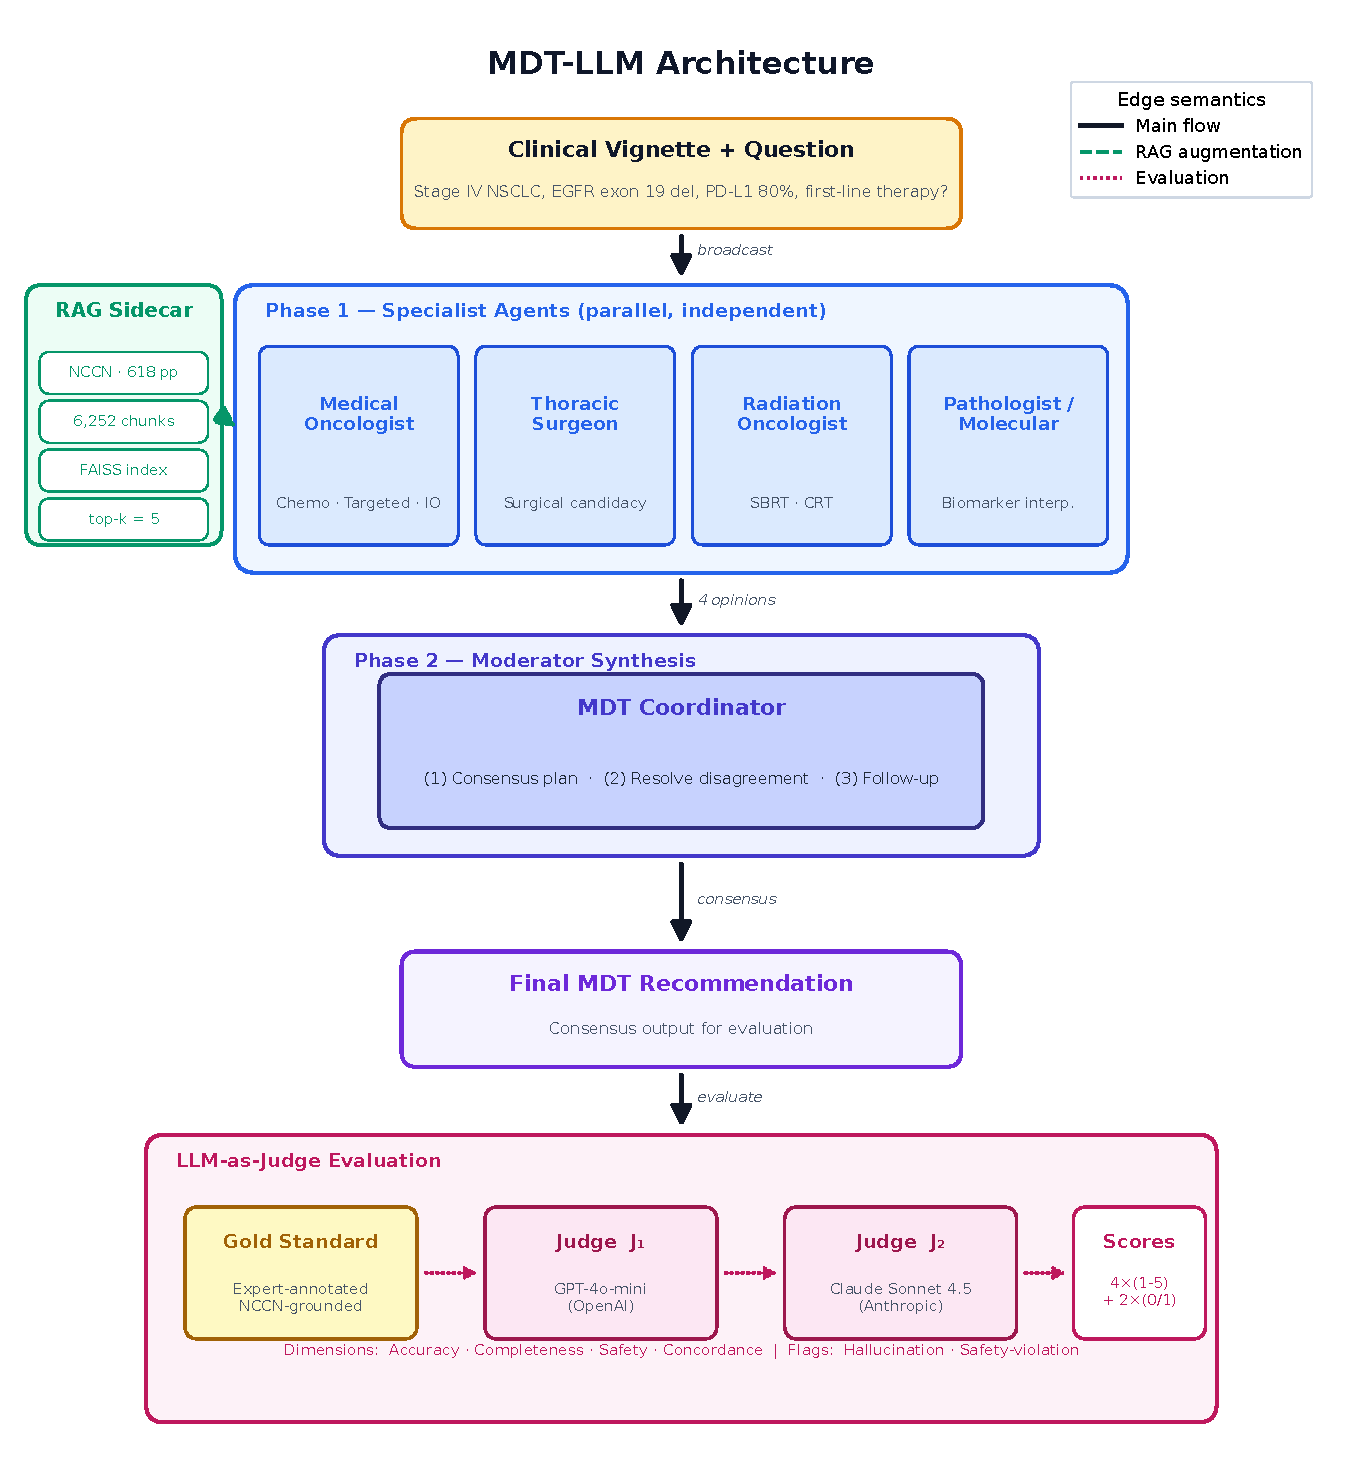
\includegraphics[width=0.92\linewidth]{fig1_architecture.pdf}
\caption{\MDTLLM{} architecture. A clinical vignette and question are
presented in parallel to four role-conditioned specialist agents, each
instantiated with a distinct system prompt. Their individual opinions
are synthesized by a moderator into a consensus recommendation. When
RAG is enabled, chunks retrieved from the NCCN guidelines (indexed in
FAISS) are injected into the context of each agent. Two LLM judges
score the output against a gold-standard answer.}
\label{fig:arch}
\end{figure*}

\subsection{Multi-agent MDT design}
\subsubsection{Role selection}
The four specialist roles match the minimum composition of a thoracic
oncology MDT as specified in the NCCN guidelines (Table~\ref{tab:roles}).

\begin{table}[!ht]
\caption{Specialist roles and primary responsibilities.}
\label{tab:roles}
\centering
\small
\begin{tabular}{lll}
\toprule
Agent & Role & Primary responsibility \\
\midrule
$A_1$ & Medical Oncologist & Systemic therapy (chemo/targeted/IO) \\
$A_2$ & Thoracic Surgeon & Surgical candidacy; perioperative \\
$A_3$ & Radiation Oncologist & Definitive/adjuvant/palliative/SBRT \\
$A_4$ & Pathologist / Molecular & Histology; biomarker interpretation \\
\bottomrule
\end{tabular}
\end{table}

Each agent is instantiated by prompting the underlying LLM with a
role-specific system message; full prompts are provided in
Appendix~\ref{app:prompts}.

\subsubsection{Two-phase orchestration}
\textbf{Phase 1: Independent specialist opinions.} The four agents
receive the scenario \emph{in parallel}; specialists cannot see each
other's outputs at this phase, mirroring pre-meeting preparation in
real MDT. \textbf{Phase 2: Moderator synthesis.} A fifth agent $M$
receives all four opinions concatenated with the original case and
produces: (i) the agreed treatment plan with specific drugs, doses,
schedules; (ii) explicit disagreement resolution; (iii) follow-up and
monitoring recommendations; (iv) guideline citations.

\subsubsection{Homogeneous vs.\ heterogeneous agents}
In the main study we use a homogeneous configuration: all five agents
are instantiated from the same underlying LLM, differentiated only by
role-specific system prompts. The heterogeneous variant
(Section~\ref{sec:hetero}) assigns different LLMs to different roles.

\subsection{Retrieval-augmented generation pipeline}
\label{sec:rag}

\paragraph{Corpus.} Four NCCN clinical practice guideline documents:
NSCLC v5.2026, SCLC v2.2026, Lung Cancer Screening v2.2026, and
Management of Immune Checkpoint Inhibitor-Related Toxicities v1.2026;
total $N_p = 618$ pages, loaded via PyMuPDF.

\paragraph{Chunking.} We apply a recursive character splitter
$\mathrm{Split}: \Sigma^{*} \to \mathcal{C} = \{c_1, \ldots, c_{|\mathcal{C}|}\}$
with hierarchy $\mathcal{H} = (\texttt{\textbackslash n\textbackslash n},
\texttt{\textbackslash n}, \texttt{.~}, \texttt{~}, \epsilon)$:
\begin{equation}
\mathrm{Split}(\mathcal{D};\ \ell, o, \mathcal{H})
= \{c_i\}_{i=1}^{|\mathcal{C}|}\quad \text{s.t.}\quad |c_i| \leq \ell,\ |c_i \cap c_{i+1}| \geq o,
\label{eq:chunk}
\end{equation}
with chunk-length cap $\ell = 512$ and overlap $o = 128$ characters,
yielding $|\mathcal{C}| = 6{,}252$ chunks. The hierarchy is applied
recursively, preferring higher-level separators to preserve semantic
boundaries.

\paragraph{Dense embedding and index.} Each chunk $c_i$ and each query
$q$ is mapped to a dense vector via
$\mathbf{E}: \Sigma^{*} \to \mathbb{R}^{d}$ (OpenAI
\texttt{text-embedding-3-large}, $d = 3{,}072$). Embeddings are
$\ell_2$-normalized so that inner-product retrieval is equivalent to
cosine similarity:
\begin{equation}
\mathbf{v}_i = \frac{\mathbf{E}(c_i)}{\lVert \mathbf{E}(c_i) \rVert_2},\qquad
\mathbf{u} = \frac{\mathbf{E}(q)}{\lVert \mathbf{E}(q) \rVert_2},\qquad
\mathrm{sim}(q, c_i) = \langle \mathbf{u}, \mathbf{v}_i \rangle = \cos\theta.
\label{eq:sim}
\end{equation}
The index $\mathcal{I}$ is a FAISS \cite{Johnson2019FAISS,Douze2024FAISS}
flat inner-product structure (\texttt{IndexFlatIP}) over
$\{\mathbf{v}_i\}_{i=1}^{|\mathcal{C}|}$; exact search is feasible at
this corpus size ($|\mathcal{C}| \cdot d \approx 77$\,MB).

\paragraph{Top-$k$ retrieval.} Let $\sigma$ be a permutation of
$\{1, \ldots, |\mathcal{C}|\}$ sorting chunks by descending similarity
to query $q$. The retrieval function outputs the concatenation of the
top-$k$ chunks with source attribution:
\begin{equation}
R_k(q) = \bigoplus_{r=1}^{k} \bigl[\,\mathrm{src}(c_{\sigma(r)}),\ c_{\sigma(r)}\bigr],
\qquad k = 5 \text{ (default)},
\label{eq:topk}
\end{equation}
where $\mathrm{src}(c)$ is a bracketed tag of form
\texttt{[Source: file, Page p]}. In RAG conditions, $R_k(q)$ is
prepended to the user message of each agent call
(Eq.~\ref{eq:framework}). The top-$k$ sensitivity ablation
(\S\ref{sec:topk}) varies $k \in \{1, 3, 5, 10\}$.

\subsection{\BENCH{} benchmark}
\label{sec:bench}
\BENCH{} was constructed to satisfy four criteria: clinical realism,
guideline-groundedness, taxonomic coverage, and difficulty
stratification. It contains 100 scenarios across 6 clinical domains
$\times$ 3 difficulty levels (Table~\ref{tab:bench}).

\begin{table}[!ht]
\caption{Composition of \BENCH{} (domain $\times$ difficulty).}
\label{tab:bench}
\centering
\small
\begin{tabular}{lrrrr}
\toprule
Domain & Easy & Medium & Hard & Total \\
\midrule
D1: Diagnosis / Screening    & 5 & 6 & 6 & 17 \\
D2: Staging / Molecular      & 4 & 6 & 5 & 15 \\
D3: First-line Therapy       & 4 & 8 & 8 & 20 \\
D4: Subsequent / Resistance  & 3 & 8 & 5 & 16 \\
D5: Adverse Events           & 5 & 7 & 5 & 17 \\
D6: Follow-up                & 4 & 6 & 5 & 15 \\
\midrule
\textbf{Total}               & \textbf{25} & \textbf{41} & \textbf{34}
  & \textbf{100} \\
\bottomrule
\end{tabular}
\end{table}

Each scenario was drafted and annotated by a board-certified thoracic
oncology specialist; every gold-standard was independently verified
against NCCN v5.2026 at the time of benchmark freezing (April 2026).

\subsection{LLM-as-judge evaluation protocol}
\label{sec:judge}

\paragraph{Two-judge design.} Two judges from distinct providers are
used to reduce single-vendor bias: $J_1$ = GPT-4o-mini (OpenAI),
$J_2$ = Claude Sonnet~4.5 (Anthropic). Formally, each judge is a
mapping $J : \Sigma^{*} \times \Sigma^{*} \times \Sigma^{*} \to
\mathcal{S}$, where $\mathcal{S} = \{1,\ldots,5\}^4 \times \{0,1\}^2$
represents the four ordinal scores and two binary flags:
\begin{equation}
J(q, g, \hat y) = \bigl(s^{\mathrm{acc}}, s^{\mathrm{com}}, s^{\mathrm{saf}}, s^{\mathrm{con}}, h, v\bigr),
\label{eq:judge-signature}
\end{equation}
with components defined in Appendix~\ref{app:prompts}. Responses are
output as JSON and parsed via regex-anchored extraction; $<0.5\%$ of
calls failed parsing in our runs and were excluded.

\paragraph{Ordinal aggregation.} For each $(q, L, c)$ triple we
aggregate the two judges' ordinal dimensions to a per-dimension mean
and an overall mean score:
\begin{equation}
\bar{s}^{d}(q, L, c) = \frac{1}{2}\sum_{j=1}^{2} s^{d}_{j}(q, L, c),\qquad
\bar{s}^{\text{overall}}(q, L, c) = \frac{1}{4}\sum_{d \in \mathcal{D}} \bar{s}^{d}(q, L, c),
\label{eq:ensemble}
\end{equation}
where $\mathcal{D} = \{\mathrm{acc}, \mathrm{com}, \mathrm{saf}, \mathrm{con}\}$.

\paragraph{Binary aggregation (conservative OR).} For the binary
flags $h$ (hallucination) and $v$ (safety violation) we use a
\emph{conservative} aggregation: a response is flagged if \emph{any}
judge flags it, since missing a safety issue is more costly than a
false alarm:
\begin{equation}
\bar{h}(q,L,c) = \max_{j} h_j(q,L,c),\qquad
\bar{v}(q,L,c) = \max_{j} v_j(q,L,c).
\label{eq:binary-agg}
\end{equation}

\paragraph{Inter-judge reliability.} For each ordinal dimension
$d \in \mathcal{D}$, inter-judge reliability is quantified by Cohen's
weighted $\kappa$ \cite{Cohen1968} with quadratic weights, which
accounts for the ordinal nature of the 1--5 scale:
\begin{equation}
\kappa_w(d) = 1 - \frac{\sum_{i,j} w_{ij}\, p_{ij}^{o}}{\sum_{i,j} w_{ij}\, p_{ij}^{e}},\qquad
w_{ij} = \frac{(i-j)^2}{(n-1)^2},\quad n = 5,
\label{eq:kappa}
\end{equation}
where $p_{ij}^{o}$ is the observed joint probability of $(J_1{=}i,\,J_2{=}j)$
scoring, $p_{ij}^{e} = p_{i\cdot}^{o} \cdot p_{\cdot j}^{o}$ is the
expected probability under marginal independence, and
$w_{ij} \in [0,1]$ penalizes disagreement quadratically by score
distance. A single overall $\kappa_w^{\star}$ is computed by
concatenating all ordinal dimensions:
\begin{equation}
\kappa_w^{\star} = \kappa_w\bigl(\mathrm{concat}_{d \in \mathcal{D}}\,(s_1^d, s_2^d)\bigr).
\end{equation}
We interpret $\kappa_w$ per Landis and Koch's
thresholds \cite{LandisKoch1977}: $\geq 0.81$ almost perfect,
$0.61$--$0.80$ substantial, $0.41$--$0.60$ moderate, $\leq 0.40$
fair-to-poor.

\subsection{Implementation}
Python 3.13; \texttt{openai} v2.32, \texttt{anthropic} v0.95,
LangChain \cite{LangChain2023} via \texttt{langchain\_community} for
document loading and splitting, \texttt{faiss-cpu}
v1.13~\cite{Douze2024FAISS}, \texttt{pymupdf}
v1.27~\cite{Artifex_PyMuPDF}; text embeddings via OpenAI
\texttt{text-embedding-3-large} \cite{OpenAIEmbeddings2024}, whose
performance on biomedical retrieval tasks is characterized by MTEB
\cite{MTEB2023}. All LLM calls use temperature~0 and
\texttt{max\_tokens}~1024. Full hyperparameters and release artifacts
are in Section~\ref{sec:repro}.

% ==============================================================
\section{Experimental Setup}
\label{sec:setup}

\subsection{Models evaluated}
\begin{table}[!ht]
\caption{LLMs evaluated in this study.}
\label{tab:models}
\centering
\small
\begin{tabular}{lll}
\toprule
Label & Model ID & Category \\
\midrule
GPT-4o-mini \cite{GPT4oMini} & \texttt{gpt-4o-mini-2024-07-18} & Proprietary, cost-efficient \\
Claude Sonnet 4.5 \cite{ClaudeSonnet45} & \texttt{claude-sonnet-4-5-20250929} & Proprietary, frontier \\
DeepSeek R1 \cite{DeepSeekR1} & \texttt{deepseek-reasoner} & Reasoning-specialized \\
Llama-3.3-70B \cite{Llama33} & \texttt{Llama-3.3-70B-Instruct-Turbo} & Open-weight \\
\bottomrule
\end{tabular}
\end{table}

We chose \textbf{GPT-4o-mini} rather than full GPT-4o for cost reasons
and to represent the cost-efficient tier of the OpenAI model family;
the same architectural choice rationale applies as for Llama-3.3-70B
(open-weight tier). Comparison with the frontier GPT-4o variant is a
natural extension of this work.

\subsection{Conditions}
A 2$\times$2 factorial design: \{single, MDT\} $\times$ \{zero-shot,
RAG\} = 4 conditions. Total: 4 conditions $\times$ 4 models $\times$
100 questions = 1{,}600 model responses; 2 judges yield 3{,}200 judge
scores for the main study.

\subsection{Statistical analysis}
\label{sec:stats}

\paragraph{Paired Wilcoxon signed-rank tests.} Given two paired samples
$\{a_i\}_{i=1}^{n}$ and $\{b_i\}_{i=1}^{n}$ (here, scores of a single
condition vs.\ the single zero-shot baseline, paired at the
question-level), we test $H_0{:}\ \mathrm{median}(a-b) = 0$ via
\begin{equation}
W^{+} = \sum_{i=1}^{n} \mathbb{I}(a_i - b_i > 0) \cdot \mathrm{rank}\bigl(|a_i - b_i|\bigr),
\label{eq:wilcoxon}
\end{equation}
using two-sided $p$-values from the exact or asymptotic null
distribution \cite{Wilcoxon1945}.

\paragraph{Multiple-comparison correction.} For the main pairwise
analysis we use Bonferroni correction over $|\mathcal{L}| \times
|\mathcal{C}^{-}| = 4 \times 3 = 12$ tests (each non-baseline condition
vs.\ single zero-shot, per model):
\begin{equation}
p^{\mathrm{Bonf}}_m = \min\bigl(1,\ 12\, p_m\bigr),
\end{equation}
declaring significance at $\alpha = 0.05$. For subgroup analyses
(\S5.4--5.5) we use the Benjamini-Hochberg procedure
\cite{BenjaminiHochberg1995}: sort raw $p_{(1)} \leq \ldots \leq p_{(m)}$
and declare $H_{(i)}$ significant if
\begin{equation}
p_{(i)} \leq \frac{i}{m}\,q,\qquad q = 0.05,
\end{equation}
controlling the false-discovery rate at $q$.

\paragraph{Effect sizes (Cliff's $\delta$).} As a non-parametric
companion to $p$-values we report Cliff's $\delta$
\cite{Cliff1993}, which measures the probability that a randomly chosen
value from $a$ exceeds a randomly chosen value from $b$, minus the
reverse:
\begin{equation}
\delta = \frac{1}{n_a n_b}\sum_{i=1}^{n_a}\sum_{j=1}^{n_b}\bigl[\mathbb{I}(a_i > b_j) - \mathbb{I}(a_i < b_j)\bigr] \in [-1, 1].
\label{eq:cliff}
\end{equation}
We use Cliff's conventional thresholds: $|\delta| < 0.147$ negligible;
$[0.147, 0.330)$ small; $[0.330, 0.474)$ medium; $\geq 0.474$ large.

\paragraph{Bootstrap confidence intervals.} 95\% CIs for mean scores
are constructed via $B = 1{,}000$ non-parametric bootstrap resamples at
the question level \cite{EfronTibshirani1993}. For each model$\times$condition
cell with observed scores $\{x_1, \ldots, x_n\}$:
\begin{equation}
\hat{\theta}^{(b)} = \frac{1}{n}\sum_{i=1}^{n} x_{\tau_b(i)},\quad b = 1,\ldots,B,\quad \tau_b \sim \mathrm{Unif}(\{1,\ldots,n\}^n),
\end{equation}
with percentile CI $[\,\hat{\theta}^{(B\cdot 0.025)}_{(\cdot)},\
\hat{\theta}^{(B\cdot 0.975)}_{(\cdot)}\,]$ from the ordered bootstrap
replicates.

\paragraph{Cost-quality Pareto analysis.} For the heterogeneous
ablation, we estimate per-question API cost
$C(L, c) = \sum_{\mathrm{call} \in c} (T^{\mathrm{in}}\,\pi^{\mathrm{in}}_{L}
+ T^{\mathrm{out}}\,\pi^{\mathrm{out}}_{L})/10^{6}$ where $T^{\mathrm{in/out}}$
are tokens and $\pi^{\mathrm{in/out}}_L$ are per-million-token prices.
A configuration $(L, c)$ \emph{Pareto-dominates} $(L', c')$ iff
$\bar{s}^{\text{overall}}(L,c) \geq \bar{s}^{\text{overall}}(L',c')$
and $C(L,c) \leq C(L',c')$ with at least one strict. The Pareto front
is reported in \S\ref{sec:hetero}.

\subsection{Reproducibility \& compute}
\label{sec:repro}
All API calls use temperature~0. The benchmark CSV, agent system
prompts, judge prompt, and FAISS index are released as supplementary
materials. Total wall-clock time: $\sim$12 hours (main experiment
$\sim$7 h under 4-way per-model parallelism; main judge $\sim$1 h;
ablations $\sim$3 h). Aggregate API spend: $\sim$USD 39 across all
experiments and judge scorings.

% ==============================================================
\section{Results}
\label{sec:results}

\subsection{Overall performance}
\label{sec:overall}
Table~\ref{tab:main} summarizes mean scores across the four-dimensional
rubric for all 4 LLMs $\times$ 4 conditions (3{,}200 judge scores).
Figure~\ref{fig:overall} visualizes the mean ordinal score.

\begin{table*}[!ht]
\caption{Main results: mean scores (1--5 Likert, averaged across
judges) and binary-flag rates by model $\times$ condition. Bold
indicates the best condition per model on that dimension.}
\label{tab:main}
\centering
\small
\setlength{\tabcolsep}{4pt}
\begin{adjustbox}{max width=\linewidth}
\begin{tabular}{llcccccc}
\toprule
Model & Condition & Accuracy & Completeness & Safety & Concordance
  & Halluc.\% & Safety Viol.\% \\
\midrule
\multirow{4}{*}{Claude Sonnet 4.5}
  & Single ZS      & 4.50 & 4.50 & \textbf{4.76} & 4.48 & 4  & 3 \\
  & Single + RAG   & 4.15 & 4.08 & 4.66 & 4.16 & 6  & 7 \\
  & MDT ZS         & \textbf{4.58} & \textbf{4.68} & \textbf{4.76}
                   & \textbf{4.57} & 5  & 2 \\
  & MDT + RAG      & 4.52 & 4.64 & 4.74 & 4.50 & 5  & 2 \\
\midrule
\multirow{4}{*}{DeepSeek R1}
  & Single ZS      & 4.49 & 4.57 & \textbf{4.75} & 4.50 & 8  & 5 \\
  & Single + RAG   & 4.17 & 4.04 & 4.66 & 4.16 & 5  & 5 \\
  & MDT ZS         & \textbf{4.54} & \textbf{4.72} & 4.71 & \textbf{4.54} & 4 & 5 \\
  & MDT + RAG      & 4.44 & 4.58 & 4.68 & 4.44 & 8  & 5 \\
\midrule
\multirow{4}{*}{GPT-4o-mini}
  & Single ZS      & 3.82 & 3.61 & \textbf{4.40} & 3.82 & 5  & 7 \\
  & Single + RAG   & 3.72 & 3.53 & 4.36 & 3.72 & 6  & 6 \\
  & MDT ZS         & 3.81 & 3.89 & 4.28 & 3.80 & 10 & 10 \\
  & MDT + RAG      & \textbf{3.84} & \textbf{3.89} & 4.27 & \textbf{3.84} & 12 & 9 \\
\midrule
\multirow{4}{*}{Llama-3.3-70B}
  & Single ZS      & 3.63 & 3.62 & 4.29 & 3.63 & 7  & 13 \\
  & Single + RAG   & 3.50 & 3.34 & \textbf{4.34} & 3.50 & 6  & 7 \\
  & MDT ZS         & 3.52 & \textbf{3.68} & 4.11 & 3.54 & 12 & 16 \\
  & MDT + RAG      & \textbf{3.64} & 3.66 & 4.30 & \textbf{3.64} & 18 & 12 \\
\bottomrule
\end{tabular}
\end{adjustbox}
\end{table*}

\begin{figure}[!ht]
\centering
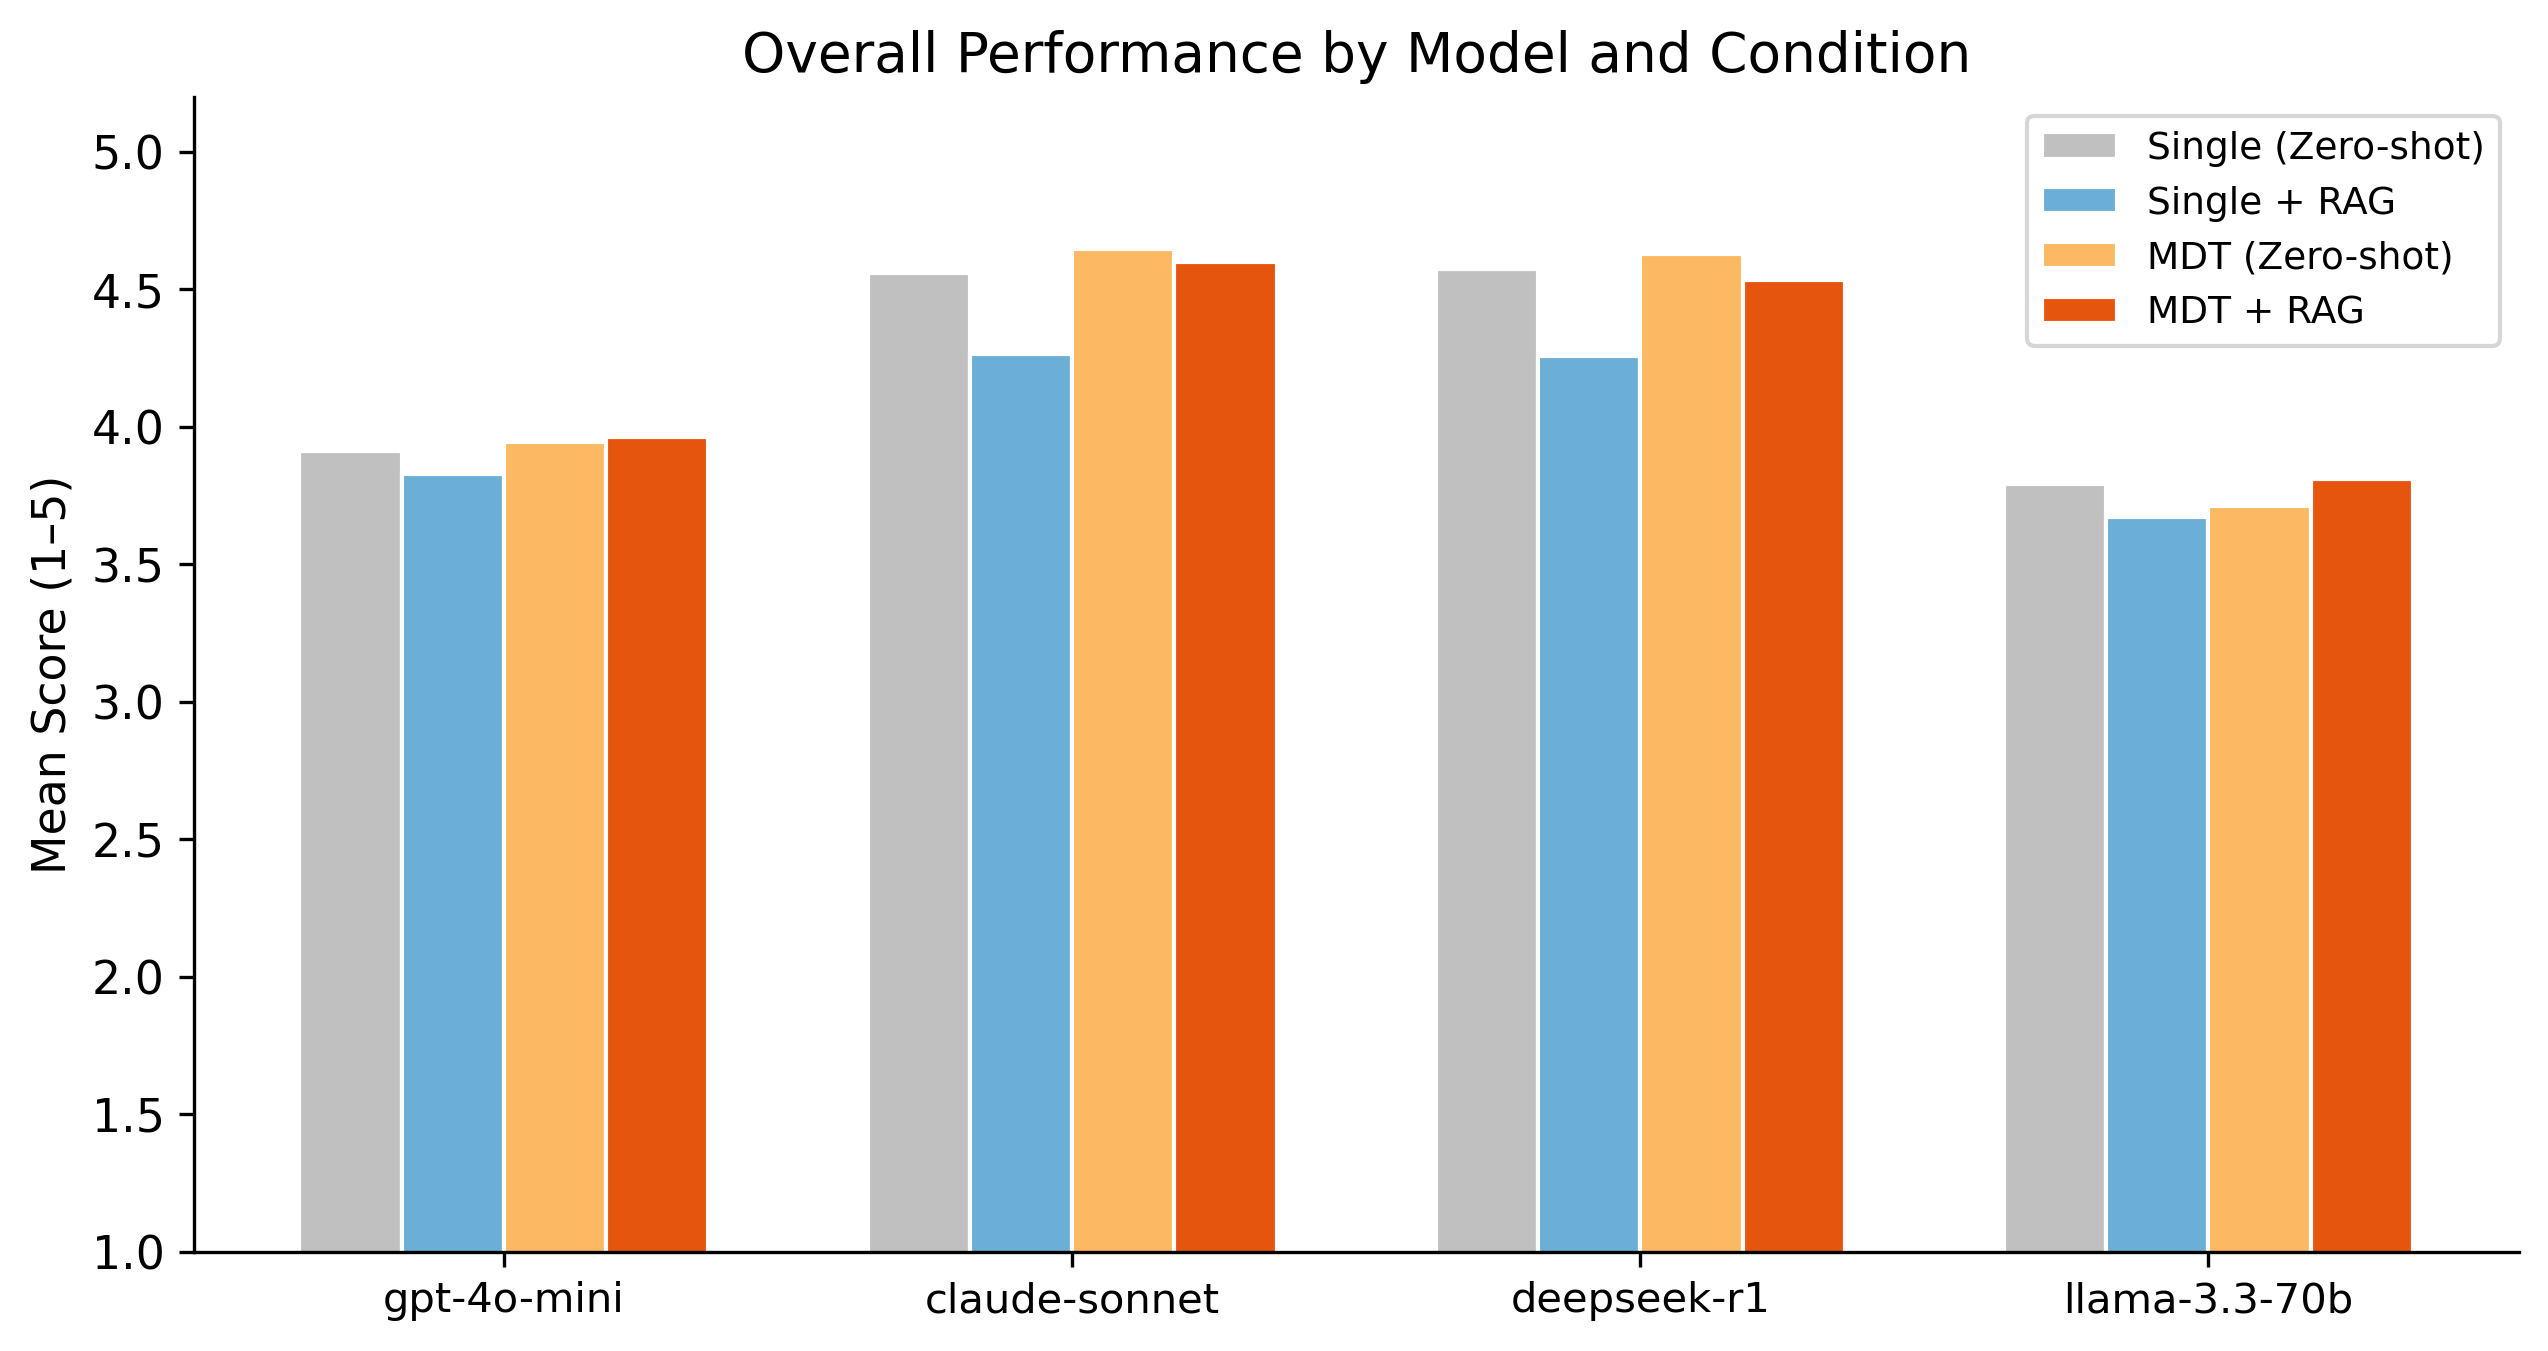
\includegraphics[width=0.95\linewidth]{fig2_overall_bar.png}
\caption{Overall performance by model $\times$ condition.}
\label{fig:overall}
\end{figure}

\subsection{Effect of retrieval augmentation: a counter-intuitive finding}
\label{sec:ragharm}
Contrary to our expectation, \textbf{retrieval augmentation consistently
reduced mean scores} relative to zero-shot baselines in all four LLMs
(Table~\ref{tab:pairwise}). The effect was statistically significant
and of medium effect size in the two strongest models after Bonferroni
correction.

\begin{table}[!ht]
\caption{Paired Wilcoxon signed-rank tests (single\_rag vs
single\_zeroshot) with Cliff's $\delta$ effect sizes and Bonferroni
correction over 12 tests.}
\label{tab:pairwise}
\centering
\small
\begin{tabular}{lcccc}
\toprule
Model & $\Delta$ mean & Wilcoxon $p$ & Bonf.\ $p$ & Cliff's $\delta$ \\
\midrule
\textbf{Claude Sonnet 4.5}  & \textbf{$-0.294$} & \textbf{0.00010}
   & \textbf{0.00122} & \textbf{$-0.283$} \\
\textbf{DeepSeek R1}        & \textbf{$-0.318$} & \textbf{0.00018}
   & \textbf{0.00210} & \textbf{$-0.356$} \\
Llama-3.3-70B               & $-0.120$ & 0.033 & 0.40 & $-0.108$ \\
GPT-4o-mini                 & $-0.081$ & 0.22  & 1.00 & $-0.043$ \\
\bottomrule
\end{tabular}
\end{table}

Several plausible mechanisms could explain this \emph{RAG-hurts-strong-%
LLMs} pattern: \emph{(a)} retrieved guideline chunks introduce
phrasing that judges compare against the more narratively-written
gold-standard, penalizing paraphrased but substantively equivalent
recommendations; \emph{(b)} retrieval noise dilutes the focused
parametric knowledge already well-encoded by strong LLMs; \emph{(c)}
NCCN guideline text is heavily represented in frontier-LLM training
corpora, making parametric recall near-optimal.

We examine mechanism \emph{(b)} via the top-$k$ ablation in
Section~\ref{sec:topk}, which rules it out by showing the harm is
present even at $k{=}1$.

\subsection{Effect of multi-agent MDT orchestration}
The overall paired comparison between MDT+RAG and single zero-shot
showed no statistically significant benefit (Claude $p{=}0.62$,
DeepSeek $p{=}0.29$, others non-significant). However,
\texttt{mdt\_zeroshot} produced the highest mean accuracy for three
of four models, suggesting the multi-agent architecture adds value
when \emph{not} confounded by the RAG-harm effect.

\subsection{Subgroup analysis by domain}
FDR-BH correction (24 tests) yielded 0 significant subgroups; 2 of 24
cells were significant at uncorrected $\alpha{=}0.05$:
\texttt{claude-sonnet} $\times$ D1 (Diagnosis/Screening, $+0.32$,
$p{=}0.04$) and \texttt{deepseek-r1} $\times$ D3 (First-line,
$+0.22$, $p{=}0.04$). Figure~\ref{fig:forest} (forest plot)
visualizes all subgroup deltas.

\begin{figure*}[!ht]
\centering
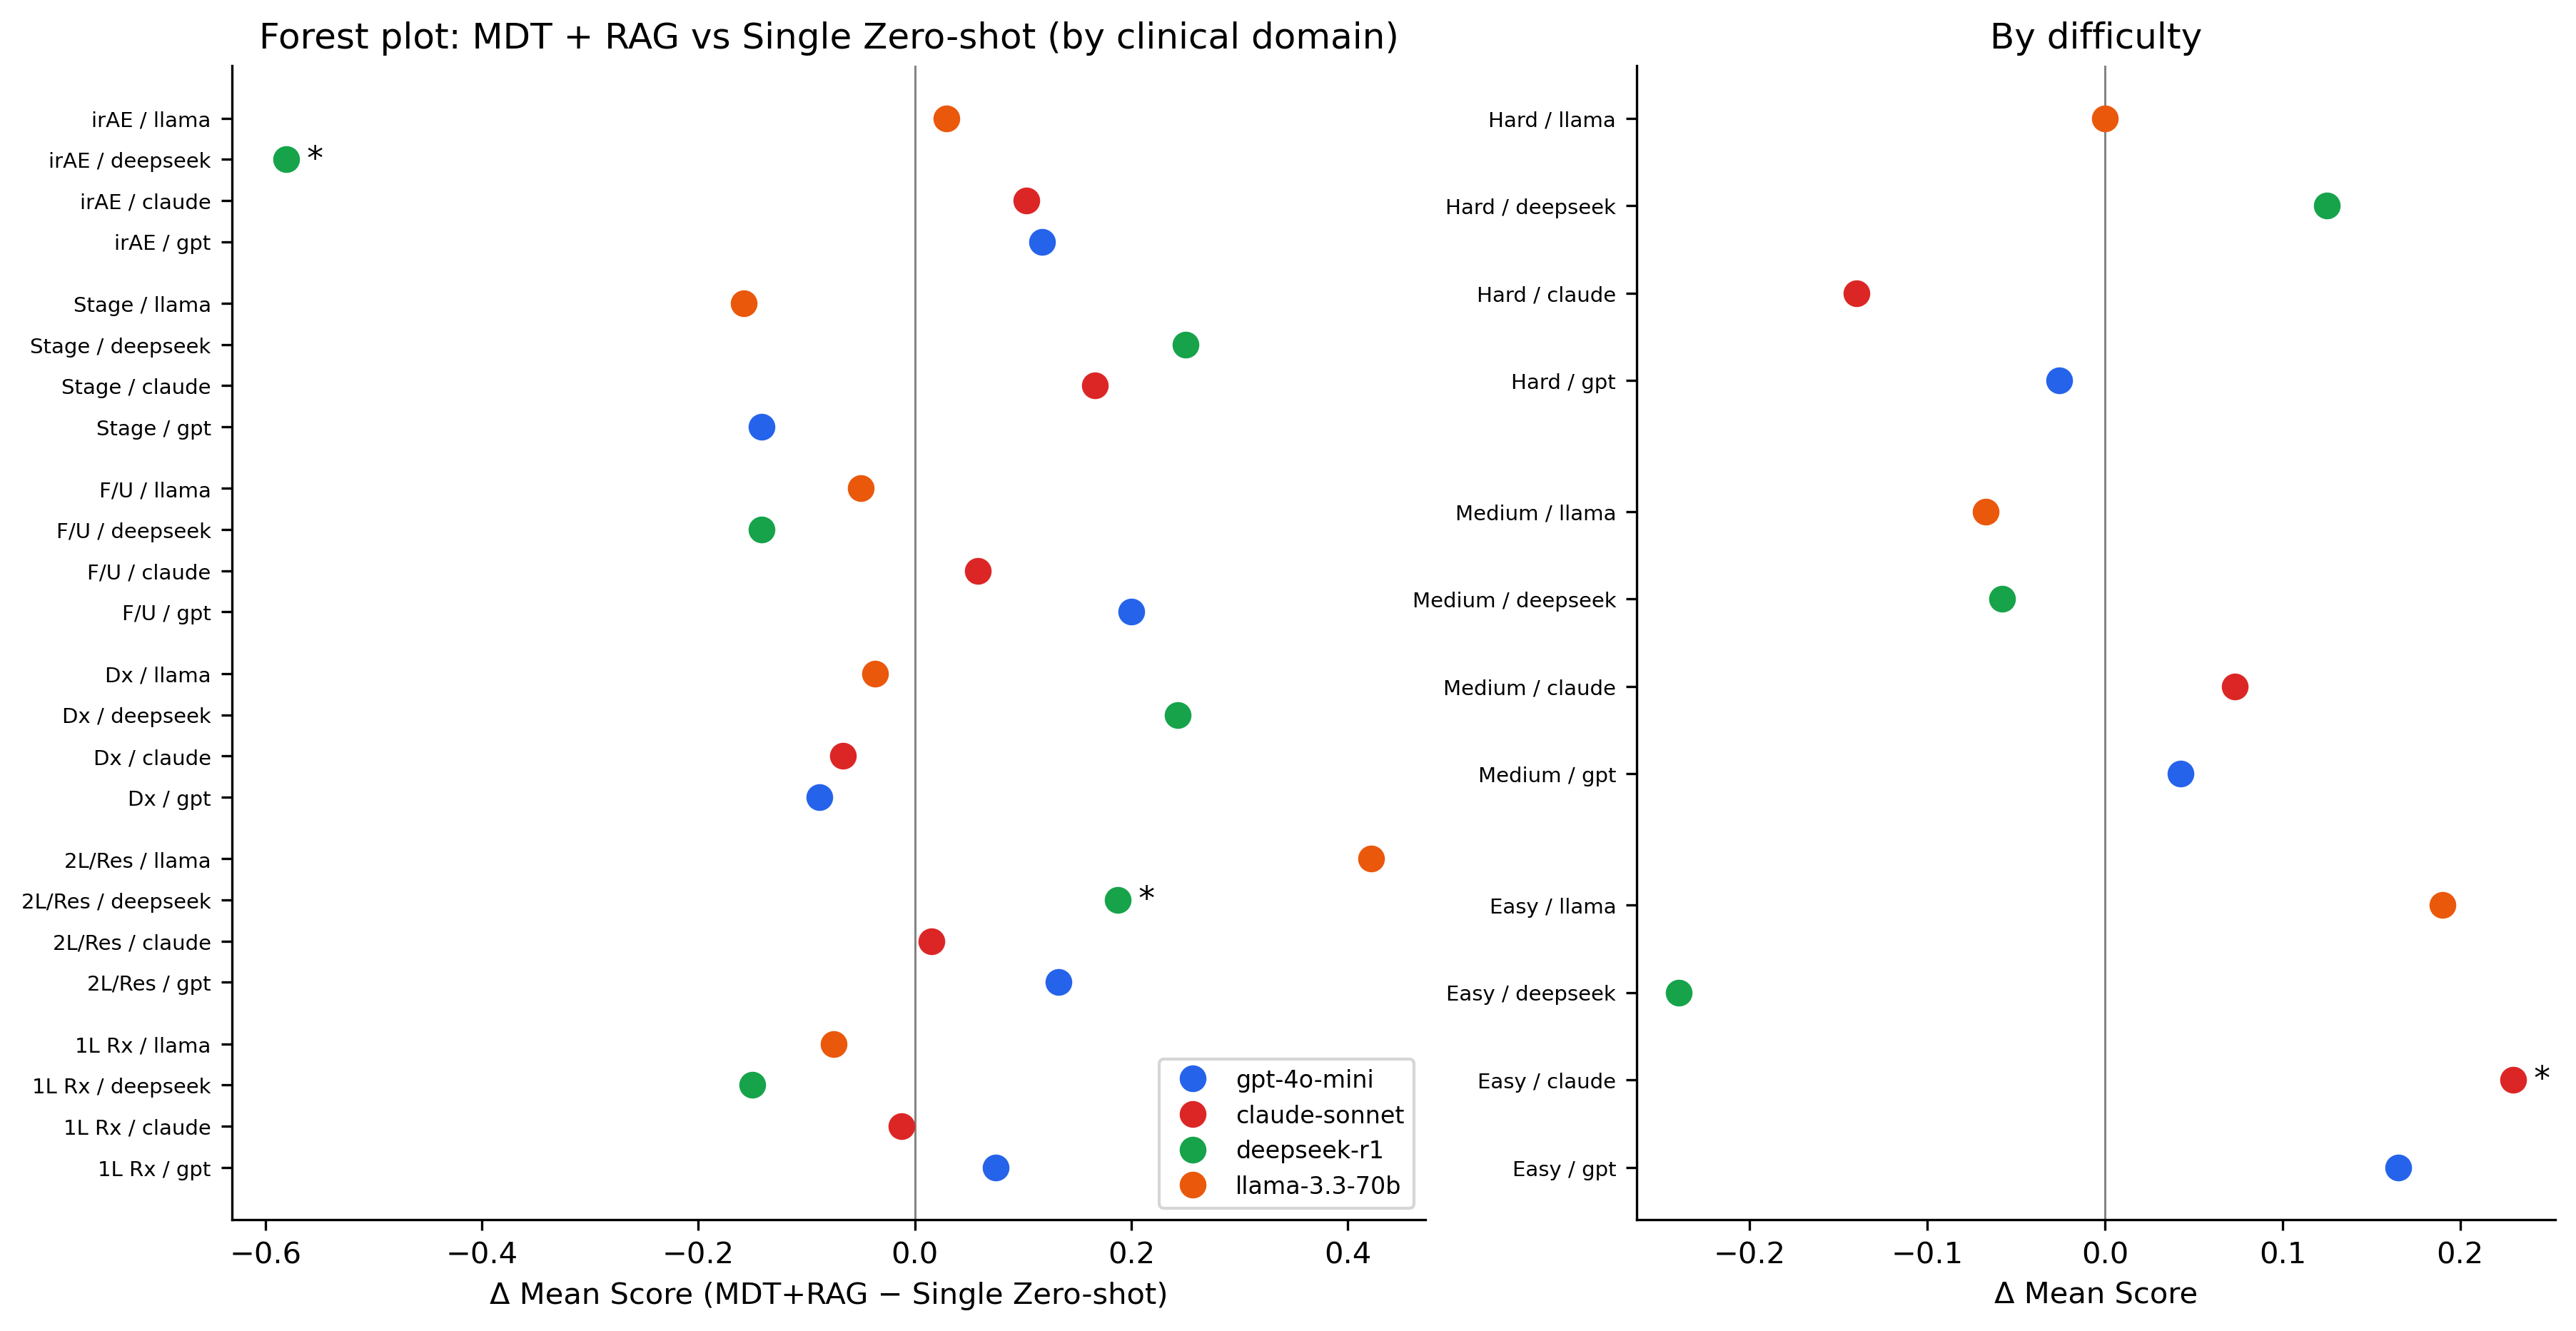
\includegraphics[width=0.92\linewidth]{fig7_forest_subgroup.png}
\caption{Forest plot: MDT+RAG vs single zero-shot across clinical
domains (left) and difficulty levels (right).}
\label{fig:forest}
\end{figure*}

\subsection{Subgroup analysis by difficulty}
For Claude Sonnet 4.5: Easy (n=25) MDT+RAG $+0.23$ ($p{=}0.023$,
$\delta{=}0.36$, medium effect); Medium (n=41) $+0.07$; Hard (n=34)
$-0.14$ (non-significant). The benefit is largest on Easy questions
and disappears on Hard ones.

\subsection{Hallucination and safety}
Hallucination rates ranged from $4\%$ (Claude Single ZS) to $18\%$
(Llama MDT+RAG). Multi-agent conditions modestly increased
hallucination for weaker models (GPT-4o-mini: $5\%\to12\%$; Llama:
$7\%\to18\%$). Figure~\ref{fig:halluc} visualizes.

\begin{figure}[!ht]
\centering
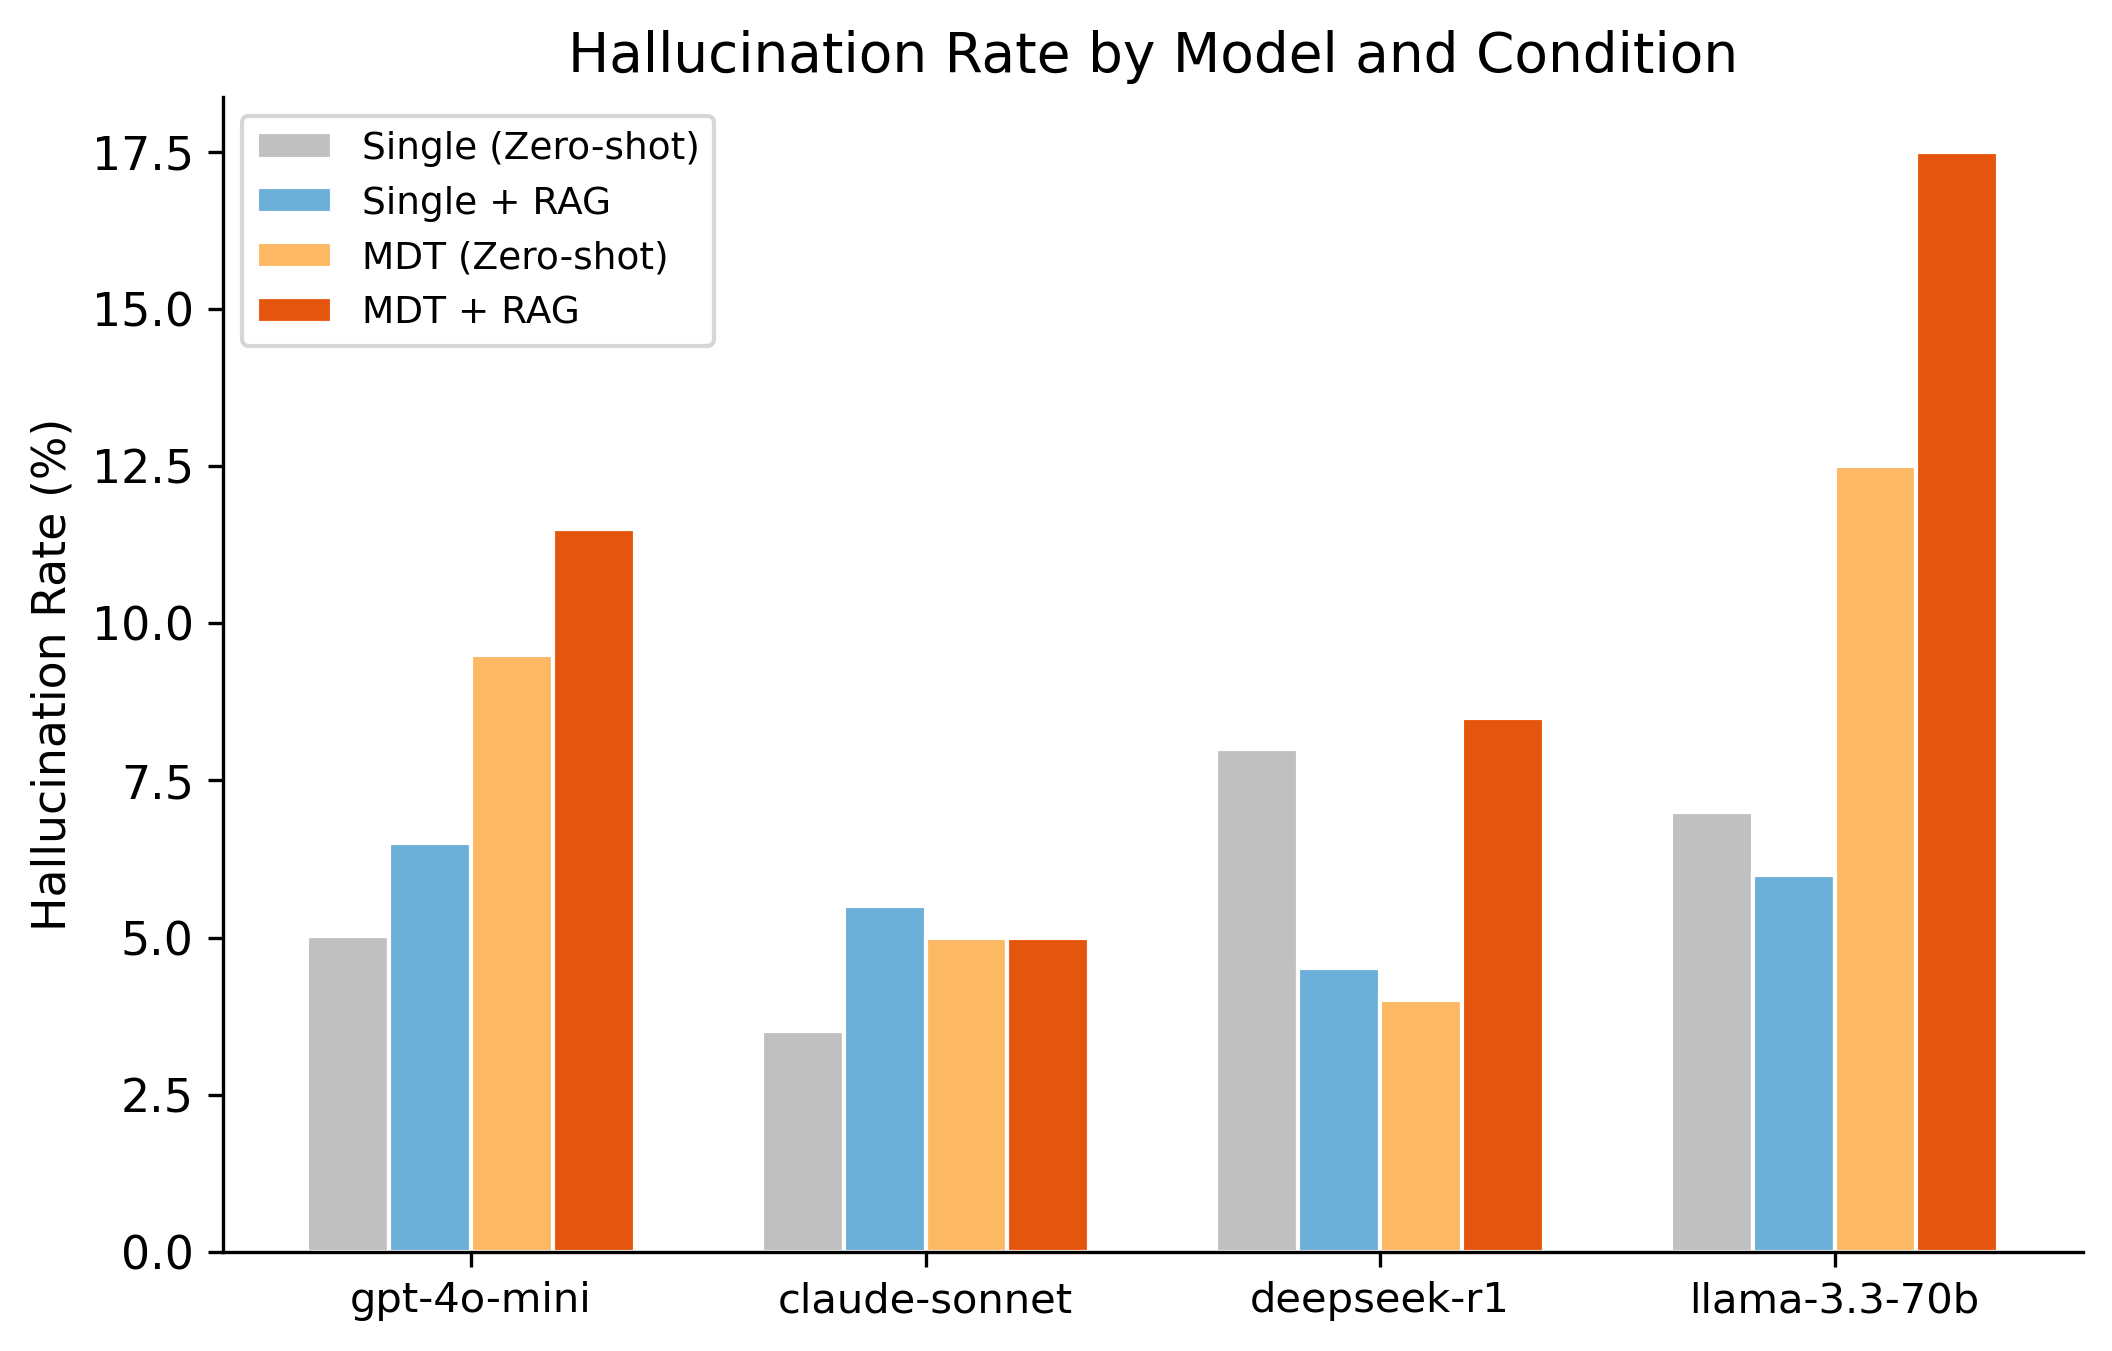
\includegraphics[width=0.9\linewidth]{fig5_hallucination.png}
\caption{Hallucination rate (at least one judge flagged) by model
$\times$ condition.}
\label{fig:halluc}
\end{figure}

\subsection{Inter-judge reliability}
\label{sec:irr}

\begin{table}[!ht]
\caption{Inter-judge reliability (Cohen's weighted $\kappa$, 1{,}600
aligned pairs).}
\label{tab:kappa}
\centering
\small
\begin{tabular}{lcc}
\toprule
Dimension & $\kappa$ & Agreement level \\
\midrule
Accuracy      & 0.699 & Substantial \\
Concordance   & 0.682 & Substantial \\
Completeness  & 0.403 & Moderate \\
Safety        & 0.208 & \textbf{Poor} \\
\midrule
Overall (concatenated) & 0.526 & Moderate \\
\bottomrule
\end{tabular}
\end{table}

Agreement is high on factual dimensions (accuracy, concordance) and
poor on safety ($\kappa{=}0.21$), suggesting that safety is a construct
on which cross-provider judges systematically disagree---motivating
methodological reformulation (binary safety-flag rather than 1--5
ordinal) in future clinical LLM benchmarks.

\subsection{Cost--accuracy trade-off}
Figure~\ref{fig:cost} plots estimated per-question API cost against
mean score. DeepSeek R1 single zero-shot achieves parity with Claude
zero-shot at approximately $1/5$ the cost.

\begin{figure}[!ht]
\centering
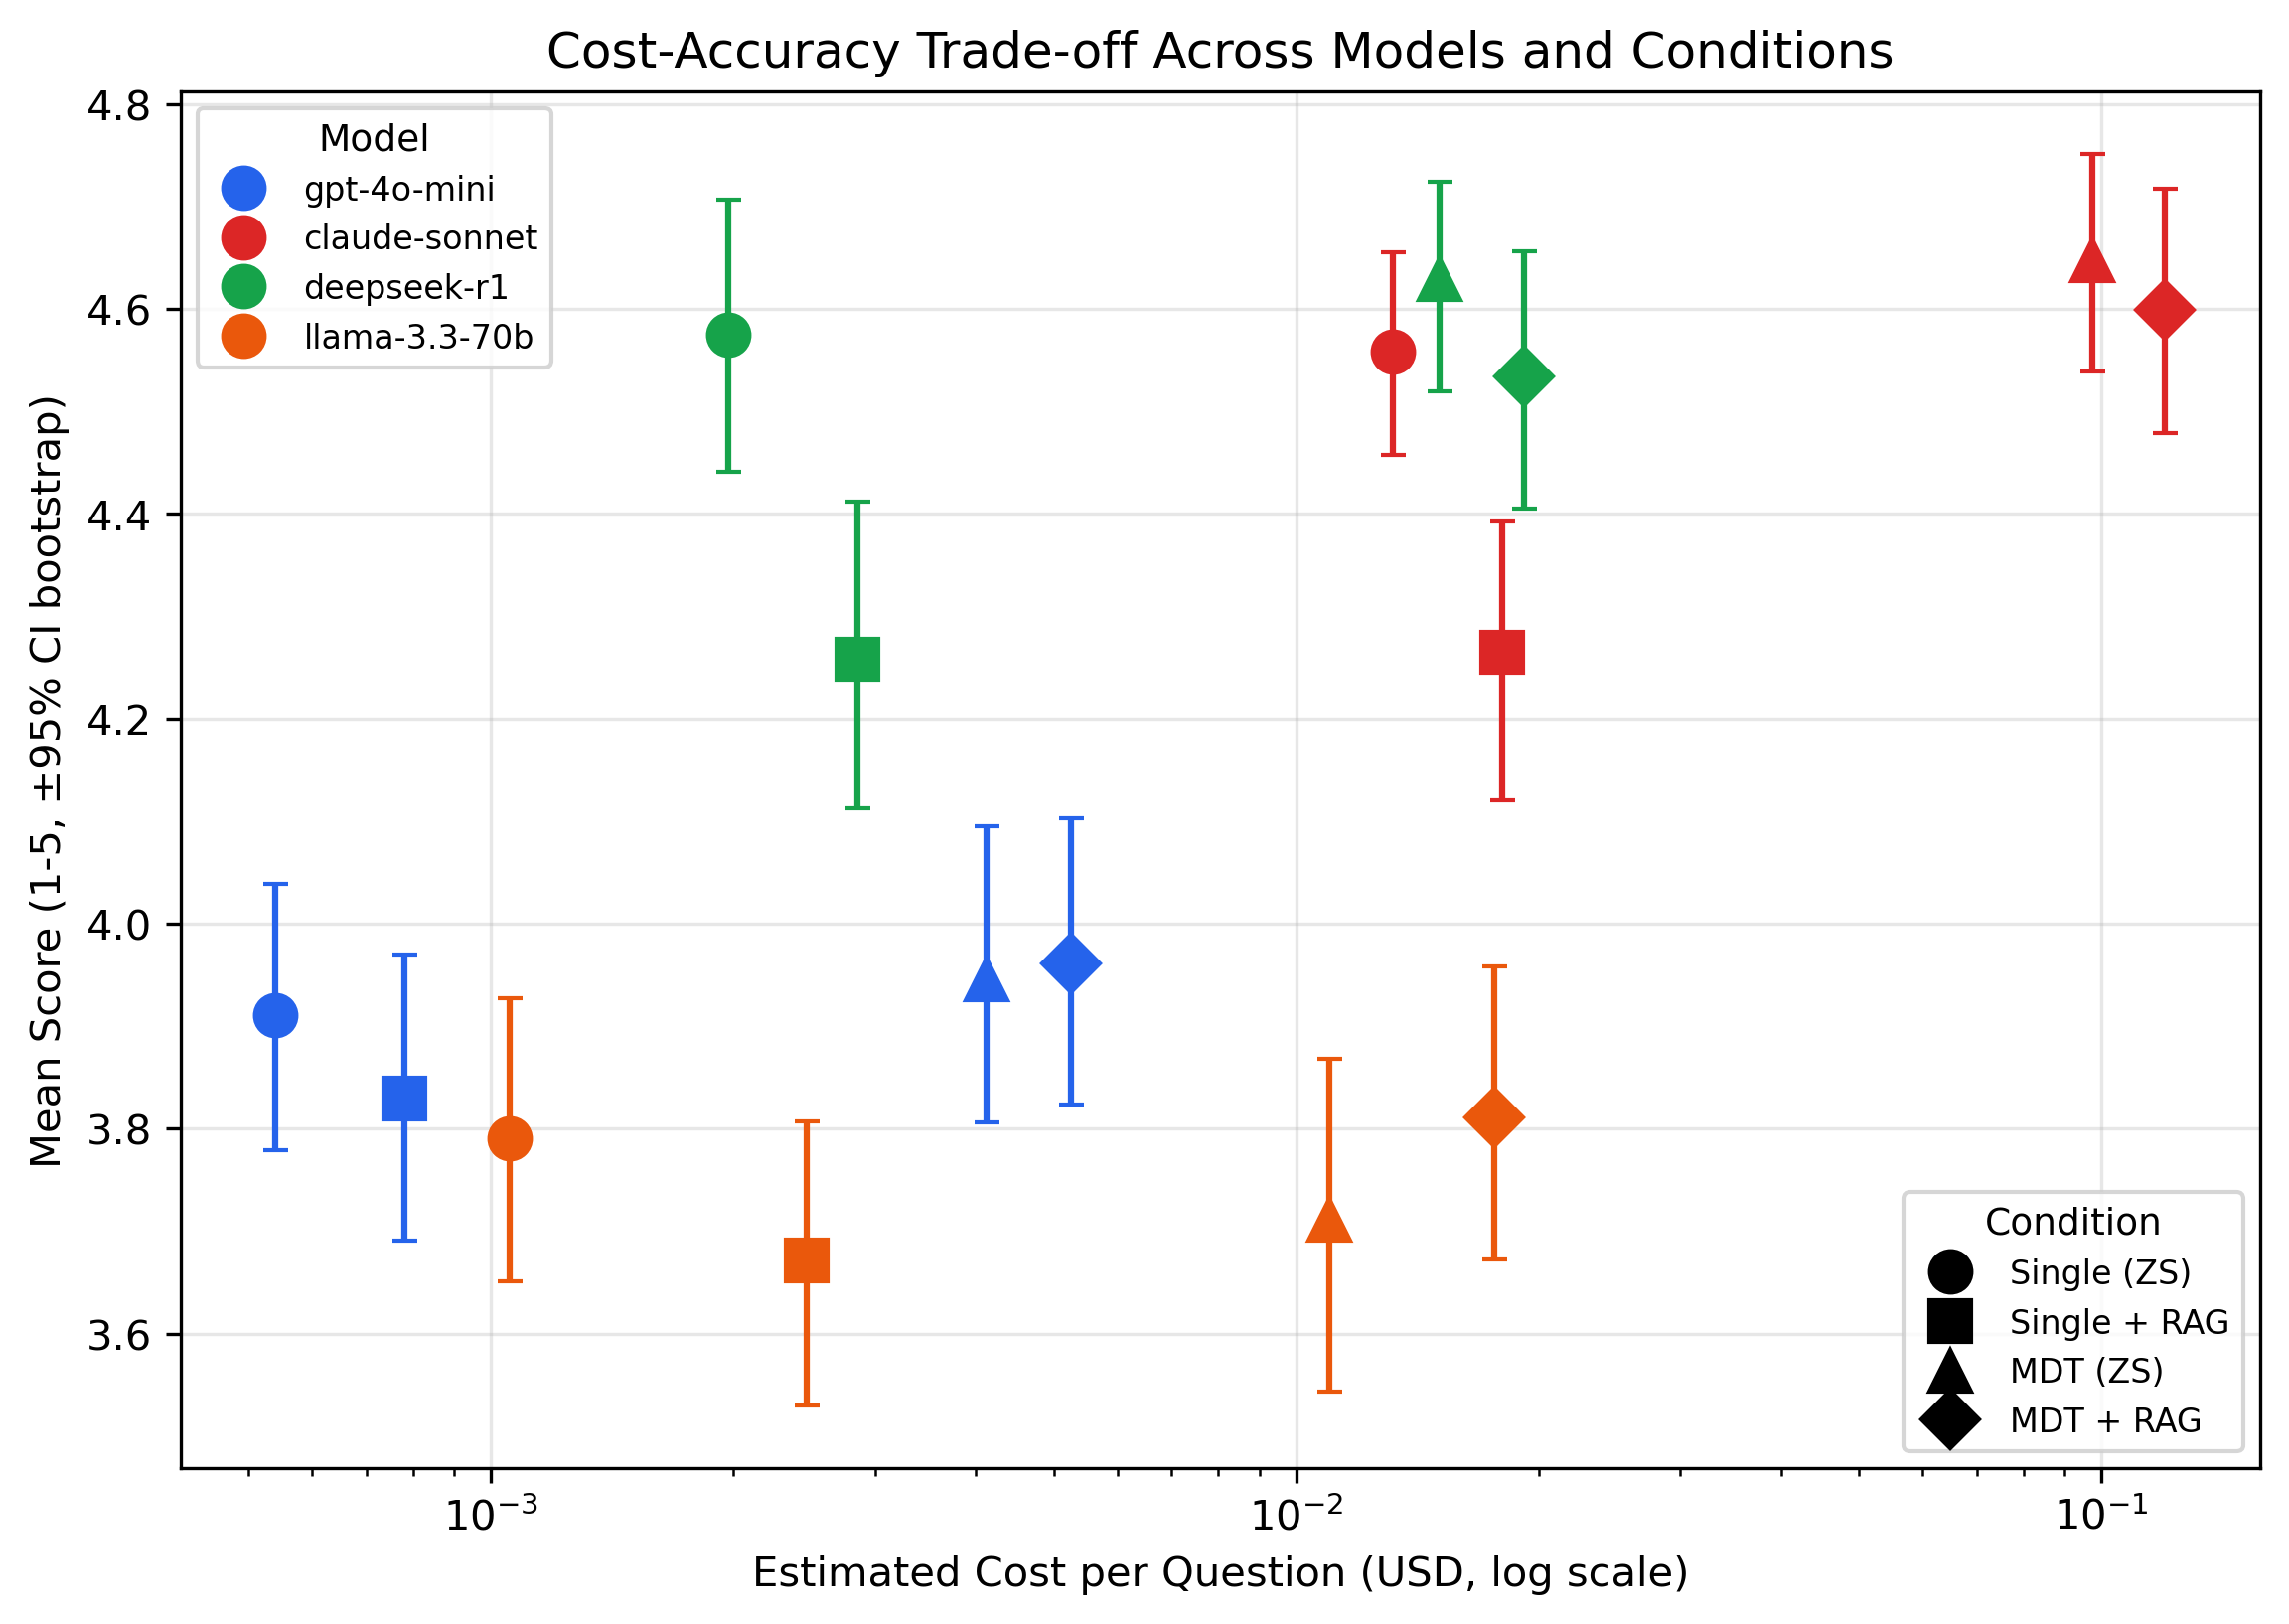
\includegraphics[width=0.95\linewidth]{fig8_cost_accuracy.png}
\caption{Cost--accuracy trade-off across models and conditions.}
\label{fig:cost}
\end{figure}

\subsection{Ablation: RAG retrieval depth ($k$)}
\label{sec:topk}

\begin{table}[!ht]
\caption{RAG top-$k$ sensitivity on Claude Sonnet 4.5 and DeepSeek R1
(GPT-4o-mini judge, $n{=}100$ per cell).}
\label{tab:topk}
\centering
\small
\begin{tabular}{lccccc}
\toprule
Model & ZS & $k{=}1$ ($\Delta$) & $k{=}3$ ($\Delta$) & $k{=}5$ ($\Delta$)
       & $k{=}10$ ($\Delta$) \\
\midrule
Claude Sonnet 4.5 & 4.702 & 4.558 ($-0.145$) & 4.510 ($-0.192$)
  & 4.492 ($-0.210$) & 4.503 ($-0.200$) \\
DeepSeek R1       & 4.770 & 4.635 ($-0.135$) & 4.622 ($-0.147$)
  & 4.513 ($-0.257$) & 4.612 ($-0.157$) \\
\bottomrule
\end{tabular}
\end{table}

\textbf{Every $k$ value produces a score below the zero-shot baseline},
with the harm already fully manifesting at $k{=}1$
(Figure~\ref{fig:topk}). This rules out a ``retrieval overwhelm''
hypothesis and supports that even minimal guideline injection shifts
model output toward verbatim guideline phrasing---penalized by judges
comparing against the narrative gold-standard.

\begin{figure}[!ht]
\centering
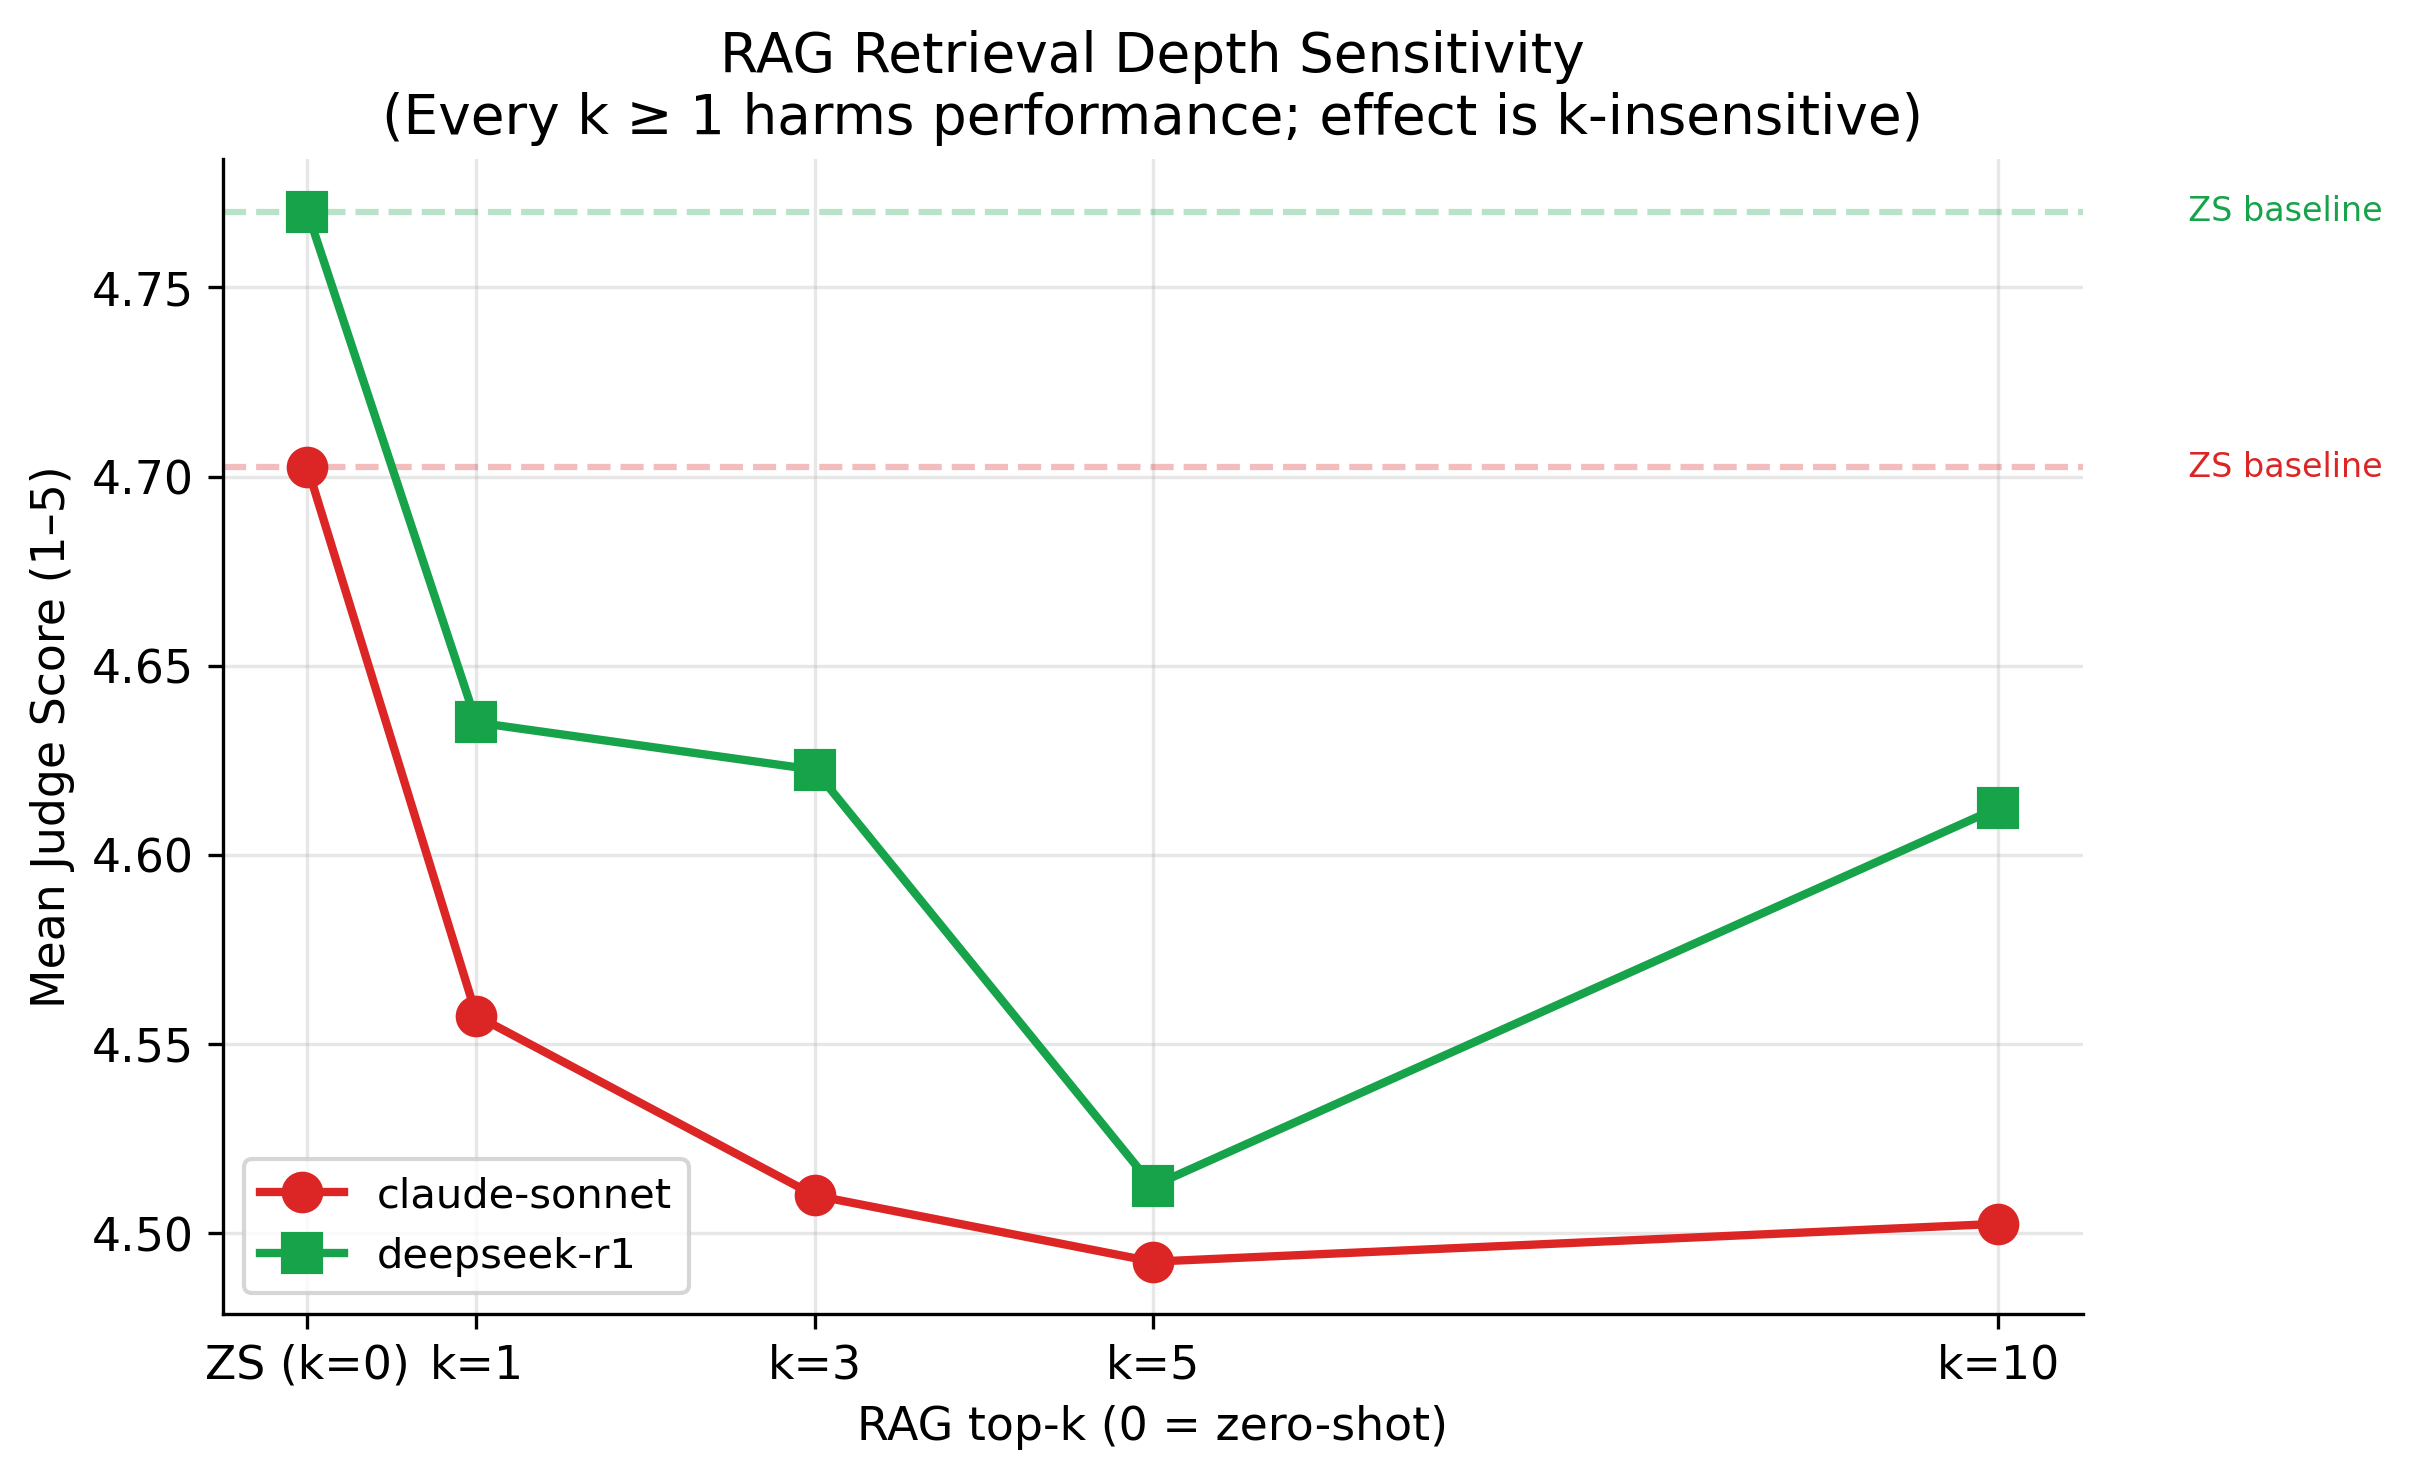
\includegraphics[width=0.88\linewidth]{fig11_rag_topk.png}
\caption{RAG top-$k$ sensitivity: all $k$ values harm performance;
effect is $k$-insensitive.}
\label{fig:topk}
\end{figure}

\subsection{Ablation: heterogeneous multi-agent configuration}
\label{sec:hetero}
We assigned each specialty to a different LLM: Claude (medical onc.),
GPT-4o-mini (surgeon), Llama-3.3-70B (rad.\ onc.), DeepSeek R1
(pathology), Claude (moderator).

\begin{table}[!ht]
\caption{Heterogeneous vs homogeneous MDT (GPT-4o-mini judge, $n{=}100$).}
\label{tab:hetero}
\centering
\small
\begin{tabular}{lccc}
\toprule
Configuration & MDT ZS & MDT+RAG & Est.\ cost/Q \\
\midrule
\textbf{Heterogeneous}      & \textbf{4.728} & \textbf{4.695}
                            & \textbf{\textasciitilde\$0.17} \\
Claude (homogeneous)        & 4.713 & 4.720 & \textasciitilde\$0.25 \\
DeepSeek R1 (homogeneous)   & 4.763 & 4.673 & \textasciitilde\$0.05 \\
GPT-4o-mini (homogeneous)   & 4.420 & 4.428 & \textasciitilde\$0.005 \\
Llama-3.3-70B (homogeneous) & 4.072 & 4.107 & \textasciitilde\$0.02 \\
\bottomrule
\end{tabular}
\end{table}

The heterogeneous MDT achieved $4.728$ in zero-shot---marginally higher
than Claude homogeneous ($+0.015$, $p{=}0.75$, not significant) and
near parity with the best homogeneous (DeepSeek, $4.763$). Most
notably, weaker models embedded in the heterogeneous ensemble
substantially outperformed their homogeneous counterparts: Llama in
hetero = $4.73$ vs.\ Llama-only MDT = $4.07$ ($\Delta{=}+0.66$). The
heterogeneous MDT is \textbf{Pareto-efficient}: $\sim32\%$ cheaper
than Claude homogeneous at equivalent accuracy
(Figure~\ref{fig:hetero}).

\begin{figure}[!ht]
\centering
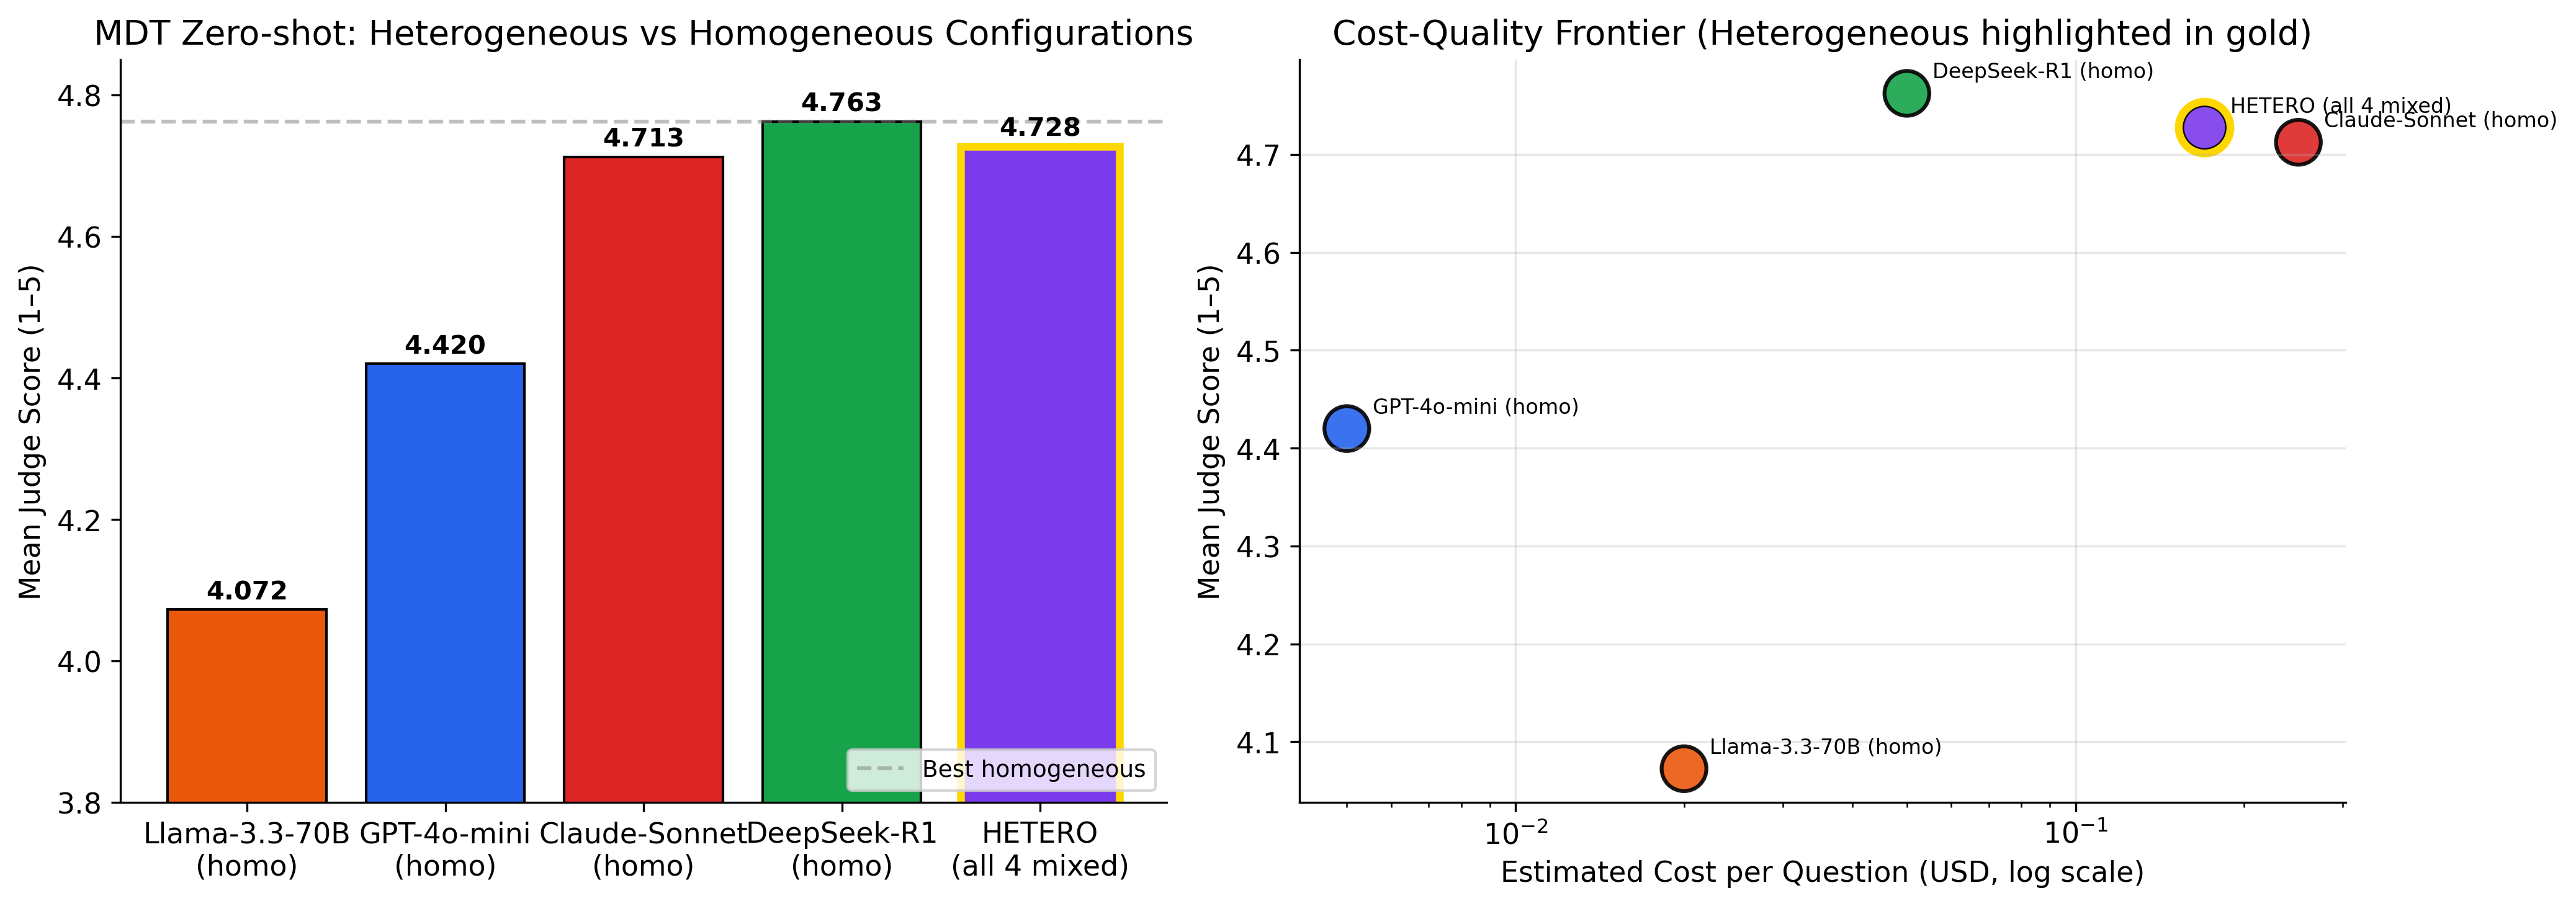
\includegraphics[width=0.98\linewidth]{fig12_heterogeneous.png}
\caption{Heterogeneous vs homogeneous MDT: mean score (left) and
cost-quality frontier (right). Heterogeneous highlighted in gold.}
\label{fig:hetero}
\end{figure}

\subsection{Error taxonomy}
\label{sec:errors}
Of the 481 low-scoring responses (mean score $<3.5$ in either judge),
we classified error types using keyword heuristics:

\begin{table}[!ht]
\caption{Error taxonomy across low-scoring responses.}
\label{tab:errors}
\centering
\small
\begin{tabular}{lcc}
\toprule
Error type & Count & \% of low-scoring \\
\midrule
No explicit guideline citation              & 181 & $37.6\%$ \\
Missing driver-mutation priority (IO w/ EGFR/ALK present) & 41 & $8.5\%$ \\
Fabricated trial name                        & 6  & $1.2\%$ \\
Vague dosing                                 & 3  & $0.6\%$ \\
\bottomrule
\end{tabular}
\end{table}

The clinically most concerning error---recommending immunotherapy in a
patient with an actionable driver mutation---occurred in $\sim9\%$ of
low-scoring outputs, posing direct patient-safety risk and motivating
automated driver-mutation-aware guardrails in any clinical deployment.

\subsection{Summary of main findings}
\begin{enumerate}
\item Naive RAG reduces output quality in strong LLMs (Claude
  $\Delta{=}-0.29$, $p{=}0.001$; DeepSeek $\Delta{=}-0.32$,
  $p{=}0.002$; Bonferroni-corrected).
\item The RAG harm is independent of retrieval depth ($k{=}1$ through
  $k{=}10$ all below baseline).
\item Multi-agent MDT produces modest non-significant gains overall,
  with benefit concentrated in Easy-to-Medium questions for Claude.
\item Heterogeneous MDT matches the best homogeneous MDT at $\sim 32\%$
  lower cost; role specialization partially compensates for individual
  model weaknesses.
\item Inter-judge $\kappa$ is substantial on factual dimensions but
  poor on safety ($\kappa{=}0.21$).
\item $8.5\%$ of low-scoring outputs recommend immunotherapy when an
  actionable driver mutation is present.
\end{enumerate}

% ==============================================================
\section{Discussion}
\label{sec:discussion}

\subsection{Principal findings and interpretation}
Our study provides the first systematic factorial benchmarking of
multi-agent LLM orchestration combined with RAG for oncology
treatment-planning decisions. Three findings stand out.

\textbf{First}, retrieval augmentation \emph{reduced} clinical answer
quality of the two strongest LLMs, with statistically significant and
medium-effect-size harm (Claude $\Delta{=}-0.29$, DeepSeek
$\Delta{=}-0.32$; both Bonferroni-corrected $p<0.002$; Cliff's $\delta$
$-0.28$ and $-0.36$). The effect was robust to retrieval depth: $k{=}1$
through $k{=}10$ all produced scores below the zero-shot baseline.
This rules out a ``too-much-context'' explanation and implicates the
mechanism of guideline injection itself: forcing a well-pretrained LLM
to quote retrieved chunks appears to shift its output from integrated
clinical reasoning toward verbatim guideline recital, penalized by
judges comparing against narratively-phrased gold-standards.

\textbf{Second}, multi-agent MDT orchestration produced modest but
non-significant overall gains, with suggestive benefits concentrated
in Easy-to-Medium questions for the strongest model. Notably,
\texttt{mdt\_zeroshot} was the top-scoring condition for both Claude
and DeepSeek---the multi-agent benefit exists but is partially masked
when RAG is included.

\textbf{Third}, DeepSeek R1 matched or exceeded Claude Sonnet 4.5 on
this benchmark at approximately $1/5$ the API cost, and open-weight
Llama-3.3-70B under MDT+RAG approached GPT-4o-mini single zero-shot.
The architectural choice (MDT vs.\ single, RAG vs.\ zero-shot) thus
has a larger practical impact on Pareto-efficient deployment than
flagship-model selection.

\subsection{Why RAG \emph{hurts} strong LLMs}
Three mechanisms are consistent with the observed pattern:

\textbf{(i) Phrasing distortion.} Strong LLMs without retrieval produce
integrated clinical narratives. When retrieved NCCN chunks are
injected, the model tends to quote them, and judges---scoring against
a narrative gold-standard---penalize the quote-style output even when
it is factually equivalent.

\textbf{(ii) Parametric knowledge adequacy.} NCCN guidelines are
heavily represented in frontier LLM training corpora. A well-aligned
LLM already ``knows'' osimertinib is first-line for EGFR exon~19
deletion; appending a retrieved chunk adds no new signal while
displacing attention from the clinical reasoning judges value.

\textbf{(iii) Judge bias.} Our gold-standards are expert clinician
narratives, not verbatim guideline text. A RAG-augmented output
faithful to the guideline but stylistically divergent from the
gold-standard would be scored down. This would be a judge-methodology
artifact rather than a true quality degradation.

Distinguishing these mechanisms requires human expert validation on a
subset of responses, a priority for future work. Regardless of which
mechanism dominates, the practical implication is clear: naive
retrieval augmentation is not a guaranteed win for strong LLMs, and
deployments should A/B test rather than assume RAG's benefit.

\subsection{MDT $\times$ RAG interaction}
The overall MDT benefit is modest ($\Delta{\approx}+0.05$ in accuracy)
but consistent in direction. More interestingly, the MDT $\times$ RAG
interaction is \emph{negative}: adding RAG to an MDT configuration
tends to reduce scores relative to MDT alone (Claude: MDT\_ZS$=4.58$
vs MDT\_RAG$=4.52$; DeepSeek: $4.54$ vs $4.44$). This is consistent
with the phrasing-distortion interpretation---injecting retrieval into
four specialists \emph{plus} a moderator amplifies rather than
corrects the distortion, motivating future frameworks that use
retrieval more selectively (e.g., adaptive specialist-issued queries).

\subsection{Evaluation methodology insights}
The two-judge protocol yielded Cohen's weighted $\kappa$ of $0.70$
(accuracy), $0.40$ (completeness), $0.21$ (safety), $0.68$
(concordance). This gradient is consistent with construct complexity:
factual accuracy is close to a lookup task for an LLM judge, while
safety requires holistic clinical appropriateness judgment that is
subjective even among human clinicians.

Two implications follow. \emph{First}, reporting ensemble means across
judges is not a substitute for reporting the underlying $\kappa$---it
masks the degree to which subjective dimensions are under-constrained.
Future protocols should report per-dimension $\kappa$ routinely.
\emph{Second}, the safety-$\kappa$ finding motivates methodological
reformulation: binary safety-violation flags with explicit triggering
criteria may be more reproducible than 1--5 ordinal scales.

\subsection{Heterogeneous agents: role specialization as compensator}
Our heterogeneous ablation (\S\ref{sec:hetero}) shows that role-
specialized prompting compensates for underlying model weakness:
Llama-3.3-70B alone scores $4.07$ in homogeneous MDT, but embedded as
\emph{radiation oncologist} in a heterogeneous ensemble the overall
output scores $4.73$---a $+0.66$ gain. This suggests that
production-grade deployments can use cost-efficient heterogeneous
configurations (mixing cheap and expensive models across roles) to
approach flagship homogeneous performance at substantially lower cost.

\subsection{Practical deployment implications}
Our findings yield three concrete recommendations for institutions
considering LLM-based decision support:

\begin{enumerate}
\item \textbf{A/B test RAG before adopting it}: naive RAG provides no
  benefit and may harm performance for strong LLMs on guideline-heavy
  tasks.
\item \textbf{Prefer role-specialized multi-agent orchestration over
  flagship-model selection}: a heterogeneous MDT beats many
  homogeneous configurations and costs less.
\item \textbf{Require explicit guideline citation in prompts} and
  automate driver-mutation-aware guardrails: the most clinically
  dangerous error mode is recommending IO in driver-mutation-positive
  disease, occurring in $\sim9\%$ of low-scoring outputs.
\end{enumerate}

\subsection{Limitations}
\emph{Single-model homogeneous MDT} isolates role specialization from
model-level heterogeneity but may underestimate benefits of truly
heterogeneous deployments at scale. \emph{English-only, NCCN-centric};
generalization to ESMO-practice regions or other languages is untested.
\emph{Temporal scope}: guidelines frozen at April 2026; longitudinal
validation as guidelines evolve is future work. \emph{LLM-as-judge
limitations}: despite multi-judge protocol, judges may share biases
with models being evaluated; comparison against expert human scoring on
a subset remains desirable. \emph{Treatment-planning scope}: other MDT
functions (consent, patient communication, prognostic counseling) are
not tested. \emph{No prospective deployment}: evaluation is
retrospective and synthetic.

\subsection{Future work}
Heterogeneous multi-agent configurations at scale; dynamic retrieval
with specialist-issued follow-up queries; longitudinal multi-turn
scenarios; extension to breast, colorectal, and gastric oncology;
prospective clinical validation in a supervised-use pilot; judge
calibration against board-certified expert panels.

% ==============================================================
\section{Conclusion}
\label{sec:conclusion}

We presented \MDTLLM, a multi-agent LLM framework for evidence-based
clinical decision support that models the role composition and
synthesis structure of clinical multidisciplinary team meetings. Our
systematic $2{\times}2$ factorial evaluation across 4 frontier LLMs
and 100 expert-annotated lung-cancer scenarios produced three primary
findings that refine the prevailing enthusiasm for RAG-and-multi-agent
clinical LLM deployments: \emph{(i)} naive retrieval augmentation
reduces output quality in strong LLMs (Bonferroni-corrected significant
for Claude Sonnet~4.5 and DeepSeek R1, medium effect, $k$-insensitive);
\emph{(ii)} multi-agent MDT orchestration provides modest non-significant
overall gains but shows promise on easy-to-medium-difficulty cases for
the strongest model; \emph{(iii)} heterogeneous multi-agent
configurations match the best homogeneous MDT at $\sim{}32\%$ lower cost,
suggesting role specialization partially substitutes for model
capability. These findings question the assumption that ``more
augmentation is always better'' and motivate careful, empirically-
grounded evaluation of each architectural component before clinical
deployment.

We release \BENCH{} and the \MDTLLM{} implementation as open
resources to support future research, and we introduce a multi-judge
LLM-as-judge evaluation protocol with explicit inter-judge reliability
reporting as a methodological template for open-ended clinical LLM
benchmarking.

% ==============================================================
\section*{Data and code availability}
Benchmark, framework implementation, judge scoring outputs, and all
figures are released at \url{https://github.com/deepdoctor/MDT-LLM}.
Judge score CSV tables are provided as Supplementary Files S1--S5.

\section*{Declaration of competing interest}
The authors declare no competing interests.

\section*{CRediT authorship contribution statement}
\textbf{First Author}: Conceptualization, Software, Formal analysis,
Writing -- original draft. \textbf{Second Author}: Clinical case
authoring, Validation, Writing -- review \& editing.
\textbf{Senior Author}: Supervision, Writing -- review \& editing.

\section*{Acknowledgments}
The authors thank [reviewers / funding sources] for their contributions.

% ==============================================================
\appendix
\section{Agent and judge prompts}
\label{app:prompts}

Complete prompts are released with the open-source code repository.
Key excerpts appear below.

\subsection*{A.1 Specialist system prompts}
\textbf{Medical oncologist:}
\begin{quote}\small
You are a board-certified medical oncologist specializing in thoracic
oncology with 15 years of clinical experience. You focus on systemic
therapy decisions including chemotherapy, targeted therapy, and
immunotherapy. Analyze the case from a medical oncology perspective.
Provide evidence-based treatment recommendations citing specific
clinical trials and guideline references.
\end{quote}
\emph{(See supplementary code for thoracic surgeon, radiation
oncologist, and pathologist prompts.)}

\subsection*{A.2 Moderator prompt}
\begin{quote}\small
You are the MDT coordinator chairing a multidisciplinary tumor board
for lung cancer. You have received opinions from four specialists.
Synthesize their inputs into a unified, consensus-based treatment
recommendation stating: (1) the agreed treatment plan with specific
drugs/doses/schedules; (2) any points of disagreement and how they
were resolved; (3) recommended follow-up and monitoring. Cite
relevant guidelines.
\end{quote}

\subsection*{A.3 Judge prompt}
Judges receive the clinical question, gold-standard answer, and AI
response, then score on four ordinal dimensions (1--5) plus two
binary flags. Output is a single JSON object with a rationale sentence.
Full prompt in supplementary materials.

% ==============================================================
\bibliography{references}

\end{document}
